\documentclass[french]{beamer}
\usetheme[secheader]{Boadilla}
\usecolortheme[named=orange]{structure}
\usepackage[utf8]{inputenc}
\usepackage[T1]{fontenc}
\usepackage{times}
\usefonttheme{serif}
\usepackage{xkeyval}
\usepackage{todonotes}
\usepackage{amsmath,amsfonts,amssymb,amsthm}
\usepackage[acronym,toc,symbols]{glossaries}
\usepackage{subfig}
\usepackage[block=space,style=authoryear,citestyle=authoryear,sorting=nyt,sortcites=false,autopunct=true,autolang=hyphen,hyperref=true,abbreviate=false,backref=true,backend=biber,maxcitenames=1,maxbibnames=99]{biblatex}
\usepackage{diagbox}
%\usepackage[block=space,style=authoryear,citestyle=authoryear,sorting=nyt,sortcites=true,autopunct=true,autolang=hyphen,hyperref=true,abbreviate=false,backref=true,backend=biber]{biblatex}
%\usepackage[backend=biber]{biblatex}
\definecolor{macouleur}{rgb}{0.75,0.43,0.09}
\AtBeginSection[]{
{
%\setbeamercolor{background canvas}{bg=macouleur}
\begin{frame}
    \vfill
    \centering
    \begin{beamercolorbox}[sep=15pt,center,shadow=true,rounded=true]{title}
        %\usebeamerfont{title}\insertsectionhead\par
        %\frametitle{Outline for section \thesection}
        \tableofcontents[currentsection]
    \end{beamercolorbox}
    \vfill
\end{frame}
}
}
\AtBeginSubsection[]{
{
\begin{frame}
    \vfill
    \centering
    \begin{beamercolorbox}[sep=8pt,center,shadow=true,rounded=true]{title}
        \usebeamerfont{title}\insertsubsectionhead\par
        %
    \end{beamercolorbox}
    \vfill
\end{frame}
}
}

\addbibresource{../bibliography.bib} % BibTeX bibliography file
\defbibheading{bibempty}{}



%%%%%%%%%%%%%%%%%%%%%%%%%%%%
% Paper dependent stuff    %
%%%%%%%%%%%%%%%%%%%%%%%%%%%%


\newcommand{\ov}{\overline}
\newcommand{\oa}{\ov{a}}
%\newcommand{\oQ}{\ov{Q}}
%\newcommand{\oR}{\ov{R}}
\newcommand{\ox}{\ov{x}}
\newcommand{\oz}{\ov{z}}
\newcommand{\oy}{\ov{y}}
\newcommand{\os}{\ov{s}}
%\newcommand{\or}{\ov{r}}
%\newcommand{\ocS}{\ov{\cS}}
\newcommand{\ocF}{\ov{\cF}}
%\newcommand{\augmentedtransition}{\ov{\transition}
%\newcommand{\ocA}{\ov{\cA}}

%%%%%%%%%%%%%%%%%%%%%%%%%%%%rans
% Aesthetics               %
% over-underline, hat, bold%
%%%%%%%%%%%%%%%%%%%%%%%%%%%%

\newcommand{\eps}{\varepsilon}
\newcommand{\vareps}{\varepsilon}
\renewcommand{\epsilon}{\varepsilon}
%\renewcommand{\hat}{\widehat}
\renewcommand{\tilde}{\widetilde}
\renewcommand{\bar}{\overline}

\newcommand*{\MyDef}{\mathrm{\scriptscriptstyle def}}
\newcommand*{\eqdefU}{\ensuremath{\mathop{\overset{\MyDef}{=}}}}% Unscaled version
\newcommand*{\eqdef}{\mathop{\overset{\MyDef}{\resizebox{\widthof{\eqdefU}}{\heightof{=}}{=}}}}


\def\:#1{\protect \ifmmode {\mathbf{#1}} \else {\textbf{#1}} \fi}
\newcommand{\CommaBin}{\mathbin{\raisebox{0.5ex}{,}}}

\newcommand{\wt}[1]{\widetilde{#1}}
\newcommand{\wh}[1]{\widehat{#1}}
\newcommand{\wo}[1]{\overline{#1}}
\newcommand{\wb}[1]{\overline{#1}}

% bf and bm missing due to conflict!!
\newcommand{\bsym}[1]{\mathbf{#1}}
\newcommand{\bzero}{\mathbf{0}}
\newcommand{\ba}{\mathbf{a}}
\newcommand{\bb}{\mathbf{b}}
\newcommand{\bc}{\mathbf{c}}
\newcommand{\bd}{\mathbf{d}}
\newcommand{\be}{\mathbf{e}}
\newcommand{\bg}{\mathbf{g}}
\newcommand{\bh}{\mathbf{h}}
\newcommand{\bi}{\mathbf{i}}
\newcommand{\bj}{\mathbf{j}}
\newcommand{\bk}{\mathbf{k}}
\newcommand{\bl}{\mathbf{l}}
\newcommand{\bn}{\mathbf{n}}
%\newcommand{\bo}{\mathbf{o}}
\newcommand{\bp}{\mathbf{p}}
\newcommand{\bq}{\mathbf{q}}
\newcommand{\br}{\mathbf{r}}
\newcommand{\bs}{\mathbf{s}}
\newcommand{\bt}{\mathbf{t}}
\newcommand{\bu}{\mathbf{u}}
\newcommand{\bv}{\mathbf{v}}
\newcommand{\bw}{\mathbf{w}}
\newcommand{\bx}{\mathbf{x}}
\newcommand{\by}{\mathbf{y}}
\newcommand{\bz}{\mathbf{z}}

\newcommand{\bA}{\mathbf{A}}
\newcommand{\bB}{\mathbf{B}}
\newcommand{\bC}{\mathbf{C}}
\newcommand{\bD}{\mathbf{D}}
\newcommand{\bE}{\mathbf{E}}
\newcommand{\bF}{\mathbf{F}}
\newcommand{\bG}{\mathbf{G}}
\newcommand{\bH}{\mathbf{H}}
\newcommand{\bI}{\mathbf{I}}
\newcommand{\bJ}{\mathbf{J}}
\newcommand{\bK}{\mathbf{K}}
\newcommand{\bL}{\mathbf{L}}
\newcommand{\bM}{\mathbf{M}}
\newcommand{\bN}{\mathbf{N}}
\newcommand{\bO}{\mathbf{O}}
\newcommand{\bP}{\mathbf{P}}
\newcommand{\bQ}{\mathbf{Q}}
\newcommand{\bR}{\mathbf{R}}
\newcommand{\bS}{\mathbf{S}}
\newcommand{\bT}{\mathbf{T}}
\newcommand{\bU}{\mathbf{U}}
\newcommand{\bV}{\mathbf{V}}
\newcommand{\bW}{\mathbf{W}}
\newcommand{\bX}{\mathbf{X}}
\newcommand{\bY}{\mathbf{Y}}
\newcommand{\bZ}{\mathbf{Z}}

% calligraphic
\newcommand{\cf}{\mathcal{f}}
%\newcommand{\cA}{\mathcal{A}}
\newcommand{\cB}{\mathcal{B}}
\newcommand{\cC}{\mathcal{C}}
%\newcommand{\cD}{\mathcal{D}}
\newcommand{\cE}{\mathcal{E}}
\newcommand{\cF}{\mathcal{F}}
\newcommand{\cG}{\mathcal{G}}
\newcommand{\cH}{\mathcal{H}}
\newcommand{\cI}{\mathcal{I}}
\newcommand{\cJ}{\mathcal{J}}
\newcommand{\cL}{\mathcal{L}}
%\newcommand{\cM}{\mathcal{M}}
\newcommand{\cN}{\mathcal{N}}
\newcommand{\cO}{\mathcal{O}}
\newcommand{\cP}{\mathcal{P}}
\newcommand{\cQ}{\mathcal{Q}}
%\newcommand{\cR}{\mathcal{R}}
%\newcommand{\cS}{\mathcal{S}}
\newcommand{\cT}{\mathcal{T}}
%\newcommand{\cU}{\mathcal{U}}
\newcommand{\cV}{\mathcal{V}}
\newcommand{\cW}{\mathcal{W}}
\newcommand{\cX}{\mathcal{X}}
\newcommand{\cY}{\mathcal{Y}}
\newcommand{\cZ}{\mathcal{Z}}

\newcommand{\rf}{\mathscr{f}}
\newcommand{\rA}{\mathscr{A}}
\newcommand{\rB}{\mathscr{B}}
\newcommand{\rC}{\mathscr{C}}
\newcommand{\rD}{\mathscr{D}}
\newcommand{\rE}{\mathscr{E}}
\newcommand{\rF}{\mathscr{F}}
\newcommand{\rG}{\mathscr{G}}
\newcommand{\rH}{\mathscr{H}}
\newcommand{\rI}{\mathscr{I}}
\newcommand{\rJ}{\mathscr{J}}
\newcommand{\rK}{\mathscr{K}}
\newcommand{\rL}{\mathscr{L}}
\newcommand{\rM}{\mathscr{M}}
\newcommand{\rN}{\mathscr{N}}
\newcommand{\rO}{\mathscr{O}}
\newcommand{\rP}{\mathscr{P}}
\newcommand{\rQ}{\mathscr{Q}}
\newcommand{\rR}{\mathscr{R}}
\newcommand{\rS}{\mathscr{S}}
\newcommand{\rT}{\mathscr{T}}
\newcommand{\rU}{\mathscr{U}}
\newcommand{\rV}{\mathscr{V}}
\newcommand{\rW}{\mathscr{W}}
\newcommand{\rX}{\mathscr{X}}
\newcommand{\rY}{\mathscr{Y}}
\newcommand{\rZ}{\mathscr{Z}}

\newcommand{\bbf}{\mathbb{f}}
\newcommand{\bbA}{\mathbb{A}}
\newcommand{\bbB}{\mathbb{B}}
\newcommand{\bbC}{\mathbb{C}}
\newcommand{\bbD}{\mathbb{D}}
\newcommand{\bbE}{\mathbb{E}}
\newcommand{\bbF}{\mathbb{F}}
\newcommand{\bbG}{\mathbb{G}}
\newcommand{\bbH}{\mathbb{H}}
\newcommand{\bbI}{\mathbb{I}}
\newcommand{\bbJ}{\mathbb{J}}
\newcommand{\bbK}{\mathbb{K}}
\newcommand{\bbL}{\mathbb{L}}
\newcommand{\bbM}{\mathbb{M}}
\newcommand{\bbN}{\mathbb{N}}
\newcommand{\bbO}{\mathbb{O}}
\newcommand{\bbP}{\mathbb{P}}
\newcommand{\bbQ}{\mathbb{Q}}
\newcommand{\bbR}{\mathbb{R}}
\newcommand{\bbS}{\mathbb{S}}
\newcommand{\bbT}{\mathbb{T}}
\newcommand{\bbU}{\mathbb{U}}
\newcommand{\bbV}{\mathbb{V}}
\newcommand{\bbW}{\mathbb{W}}
\newcommand{\bbX}{\mathbb{X}}
\newcommand{\bbY}{\mathbb{Y}}
\newcommand{\bbZ}{\mathbb{Z}}


%%%%%%%%%%%%%%%%%%%%%%%%%%%%
% Math jargon              %
%%%%%%%%%%%%%%%%%%%%%%%%%%%%
\newcommand{\wrt}{w.r.t.\xspace}
\newcommand{\defeq}{\stackrel{\mathclap{\normalfont\mbox{\scriptscriptstyle def}}}{=}}
\newcommand{\maxund}[1]{\max\limits_{#1}}
\newcommand{\supund}[1]{\text{sup}\limits_{#1}}
\newcommand{\minund}[1]{\min\limits_{#1}}
\renewcommand{\epsilon}{\varepsilon}
\newcommand{\bigotime}{\mathcal{O}}


\DeclareMathOperator*{\argmin}{arg\,min} 
\DeclareMathOperator*{\argmax}{arg\,max} 
\DeclareMathOperator*{\cupdot}{\mathbin{\mathaccent\cdot\cup}}

%%%%%%%%%%%%%%%%%%%%%%%%%%%%
% Matrix operators         %
%%%%%%%%%%%%%%%%%%%%%%%%%%%%
\newcommand{\transp}{\mathsf{\scriptscriptstyle T}}

%%%%%%%%%%%%%%%%%%%%%%%%%%%%
% Statistic operators      %
%%%%%%%%%%%%%%%%%%%%%%%%%%%%
\newcommand{\probability}[1]{\mathbb{P}\left(#1\right)}
\newcommand{\probdist}{Pr}
\DeclareMathOperator*{\expectedvalue}{\mathbb{E}}
\DeclareMathOperator*{\variance}{\text{Var}}
\newcommand{\expectedvalueover}[1]{\expectedvalue\limits_{#1}}
\newcommand{\condbar}{\;\middle|\;}
\newcommand{\gaussdistr}{\mathcal{N}}
\newcommand{\uniformdistr}{\mathcal{U}}
\newcommand{\bernoullidist}{\mathcal{B}}

%%%%%%%%%%%%%%%%%%%%%%%%%%%%
% Algebraic Sets           %
%%%%%%%%%%%%%%%%%%%%%%%%%%%%
\newcommand{\Real}{\mathbb{R}}
\newcommand{\Natural}{\mathbb{N}}
\newcommand{\statespace}{\mathcal{X}}
\newcommand{\funcspace}{\mathcal{F}}
\newcommand{\dynaspace}{\mathcal{T}}


%\newtheorem{theorem}{Theorem}
%\newtheorem{definition}{Definition}
%\newtheorem{lemma}{Lemma}
%\newtheorem{proposition}{Proposition}
%\newtheorem{remark}{Remark}
%\newtheorem{property}{Property}
%\newtheorem{assumption}{Assumption}
%\newtheorem{conjecture}{Conjecture}


%\newacronym{RL}{RL}{Reinforcement Learning}
\newacronym[longplural={Markov Decision Processes}]{MDP}{MDP}{Markov Decision Process}
\newacronym[longplural={Partially Observable Markov Decision Processes}]{POMDP}{POMDP}{Partially Observable Markov Decision Process}
\newacronym{SRS}{SRS}{Speech Recognition Score}
\newacronym{SER}{SER}{Sentence Error Rate}
\newacronym{DBN}{DBN}{Deep Belief Network}
\newacronym{VI}{VI}{Value Iteration}
\newacronym{PI}{PI}{Policy Iteration}
\newacronym{SGD}{SGD}{Stochastic Gradient Descent}
\newacronym{iid}{iid}{independent and identically distributed}
\newacronym{RBM}{RBM}{Restricted Boltzmann Machine}
\newacronym{MAML}{MAML}{Model-Agnostic Meta-Learning}
%\newacronym{MOBA}{MOBA}{Multiplayer Online Battle Arena}
%\newacronym{UAV}{UAV}{Unmanned Aerial Vehicule}
%\newacronym{RTS}{RTS}{Real Time Strategy}
\newacronym{GD}{GD}{Gradient Descent}
\newacronym{LS}{LS}{Least Squares}
\newacronym{TD}{TD}{Temporal Difference}
\newacronym{FTQ}{FTQ}{Fitted-$Q$}
\newacronym{BFTQ}{BFTQ}{Budgeted Fitted-$Q$}
\newacronym{DM}{DM}{Dialogue Manager}
\newacronym{DQN}{DQN}{Deep $Q$-learning}
\newacronym{A3C}{A3C}{Asynchronous Actor-Critic Agents}
\newacronym{DRL}{DRL}{Deep Reinforcement Learning}
\newacronym{FVI}{FVI}{Fitted-Value-Iteration}
\newacronym{AVI}{AVI}{Approximate Value Iteration}
\newacronym{API}{API}{Approximate Policy Iteration}
\newacronym{PG}{PG}{Policy Gradient}
\newacronym{AC}{AC}{Actor Critic}
\newacronym{TTS}{TTS}{Text To Speech}
\newacronym{GAN}{GAN}{Generative Adversarial Network}
\newacronym{DOD}{DOD}{Department of Defense}
\newacronym{DARPA}{DARPA}{Defense Advanced Research Projects Agency}
\newacronym{HMM}{HMM}{Hidden Markov Model}
\newacronym{TL}{TL}{Transfer Learning}
\newacronym{SL}{SL}{Supervised Learning}
\newacronym{GP}{GP}{Gaussian Process}
\newacronym{SDS}{SDS}{Spoken Dialogue System}
\newacronym{NN}{NN}{Neural Network}
\newacronym{CNN}{CNN}{Convolutional Neural Network}
\newacronym[longplural={Dialogue Systems}]{DS}{DS}{Dialogue System}
%\newacronym{BUDS}{BUDS}{The Bayesian Update of Dialogue State}
\newacronym{DST}{DST}{Dialogue State Tracking}
\newacronym{DSTC}{DSTC}{Dialogue State Tracking Challenge}
\newacronym{LSPI}{LSPI}{Least Squares Policy Iteration}
\newacronym{ASR}{ASR}{Automatic Speech Recognition}
\newacronym{NDG}{NDG}{Negociation Dialogue Game}
\newacronym{UCB}{UCB}{Upper Bound Confidence}
\newacronym{ML}{ML}{Machine Learning}
\newacronym{AI}{A.I.}{Artificial Intelligence}
\newacronym{GPU}{GPU}{Graphics Processing Unit}
\newacronym{CPU}{CPU}{Central Processing Unit}
\newacronym{RNN}{RNN}{Recurrent Neural Networks}
\newacronym{LSTM}{LSTM}{Long Short-Term Memory}
\newacronym{NLG}{NLG}{Natural Language Generator}
\newacronym{NLU}{NLU}{Natural Language Understanding}
\newacronym{MIT}{MIT}{Massachusset Institute of Technology}
\newacronym[longplural={Dialogue Policies}]{DP}{DP}{Dialogue Policy}
\newacronym{MAB}{MAB}{Multi-Armed Bandit}
\newacronym{ACER}{ACER}{Actor Critic Experience Replay}
\newacronym{ER}{ER}{Experience Replay}
\newacronym{BMDP}{BMDP}{Budgeted Markov Decision Process}
\newacronym{CMDP}{CMDP}{Constrainted Markov Decision Process}
\newacronym{AGI}{AGI}{Artificial General Intelligence}
\newacronym{BVI}{BVI}{Budgeted Value Iteration}
\newacronym{REINFORCE}{REINFORCE}{REINFORCE}
\newacronym{kNN}{$k$NN}{$k$ Nearest Neighbours}
\newacronym{GUS}{GUS}{Genial Understander System}
\newacronym{VaR}{VaR}{Value at Risk}
\newacronym{CVaR}{CVaR}{Conditional Value at Risk}
\newacronym{MORL}{MORL}{Multi-Objectives Reinforcement Learning}
\newacronym{SARSA}{SARSA}{State–Action–Reward–State–Action}
%\newacronym{}{}{}
%\newacronym{}{}{}
\newcommand{\ftq}{\textrm{\textsc{FTQ}}\xspace}
\newcommand{\bftq}{\textrm{\textsc{BFTQ}}\xspace}


\newcommand{\Q}{Q}
\newcommand{\V}{V}
\newcommand{\mubot}{\mu_{\bot}}
\newcommand{\mutop}{\mu_{\top}}
\newcommand{\params}{\theta}
\newcommand{\dirac}{\delta}
\newcommand{\normal}{\mathcal{N}}
\newcommand{\binomial}{\mathcal{B}}
\newcommand{\features}{\phi}
\newcommand{\maxiteration}{K}
\newcommand{\deltastoppingcriterion}{\upsilon}
\newcommand{\extrasmallvalue}{\kappa}
\newcommand{\egreedy}{\epsilon}
\newcommand{\users}{\rU}
\newcommand{\timeslot}{\tau}
\newcommand{\cooperationrate}{\varrho}
\newcommand{\T}{N}
\newcommand{\srs}{\nu}
\newcommand{\ser}{\xi}
\newcommand{\transpose}{\top}
\newcommand{\indextransition}{i}
\newcommand{\state}{s}
\newcommand{\n}{k}
\newcommand{\learningrate}{\alpha}
\newcommand{\abo}{\overline{\mathcal{T}}}
\newcommand{\bo}{\mathcal{T}}
\newcommand{\oQ}{\overline{Q}}
\newcommand{\Qr}{Q_r}
\newcommand{\Qc}{Q_c}
\newcommand{\oR}{\overline{R}}
\newcommand{\oV}{\overline{V}}
\newcommand{\Vr}{V_r}
\newcommand{\Vc}{V_c}
\newcommand{\ocS}{\overline{\mathcal{S}}}
\newcommand{\ocA}{\overline{\mathcal{A}}}
\newcommand{\cS}{\mathcal{S}}
\newcommand{\budgetspace}{\mathscr{B}}
\newcommand{\cK}{\mathcal{K}}
\newcommand{\policies}{\overline{\Pi}}
\newcommand{\cU}{\mathcal{U}}
\newcommand{\cA}{\mathcal{A}}
\newcommand{\augmentedtransition}{\overline{P}}
\newcommand{\cD}{\mathcal{D}}
\newcommand{\reward}{R}
\newcommand{\augmentedreward}{\overline{R}}
\newcommand{\constraint}{C}
\newcommand{\transition}{P}
\newcommand{\return}{G}
\newcommand{\constraintreturn}{G_c}
\newcommand{\augmentedreturn}{\overline{G}}
\newcommand{\cM}{\mathcal{M}}
\newcommand{\policy}{\pi}
\newcommand{\budgetedpolicy}{\overline{\pi}}
\newcommand{\optimalpolicy}{\pi^*}
\newcommand{\optimalbudgetedpolicy}{\overline{\pi}^*}
\newcommand{\discountfactor}{\gamma}
\newcommand{\budgetaction}{\beta_a}
\newcommand{\nextbudget}{\beta'}
\newcommand{\budget}{\beta}
\newcommand{\projection}{\Xi}
\newcommand{\augmentedprojection}{\overline{\Xi}}

\presetkeys{todonotes}{inline}{}
\title[TITLE]{Apprentissage par renforcement pour l'optimisation des systèmes de dialogue via l'adaptation à l'utilisateur.}
\subtitle{Soutenance de thèse.}
\author{Nicolas Carrara}
\institute[ULille]{Université de Lille}
\date{Le 18 Décembre 2019}

\setbeamertemplate{footline}{%
\hfill%
\usebeamercolor[fg]{page number in head/foot}%
\usebeamerfont{page number in head/foot}%
\insertframenumber%
%\,/\,\inserttotalframenumber
\kern1em\vskip2pt%
}

\beamertemplatenavigationsymbolsempty

\begin{document}

    \begin{frame}
        \maketitle
        \centering
    \end{frame}

    \section{Introduction}

    \begin{frame}{Les sytèmes de dialogues}

        \todo{Schéma avec c'est quoi un système de dialogue}

    \end{frame}

    \begin{frame}{Trois types d'applications}

        \begin{itemize}
            \item Discussion social sans but précis.
            \item Question-Réponse
            \item Dialogues orientés tâches.
        \end{itemize}

        %C'est surtout la troisième problématique qui nous interesse.
        \todo{mettre en gras ou avant la troisème problématique}

    \end{frame}

    \begin{frame}{\textbf{Systèmes de dialogue} | sans adaptation}
        \begin{figure}
            \begin{center}
                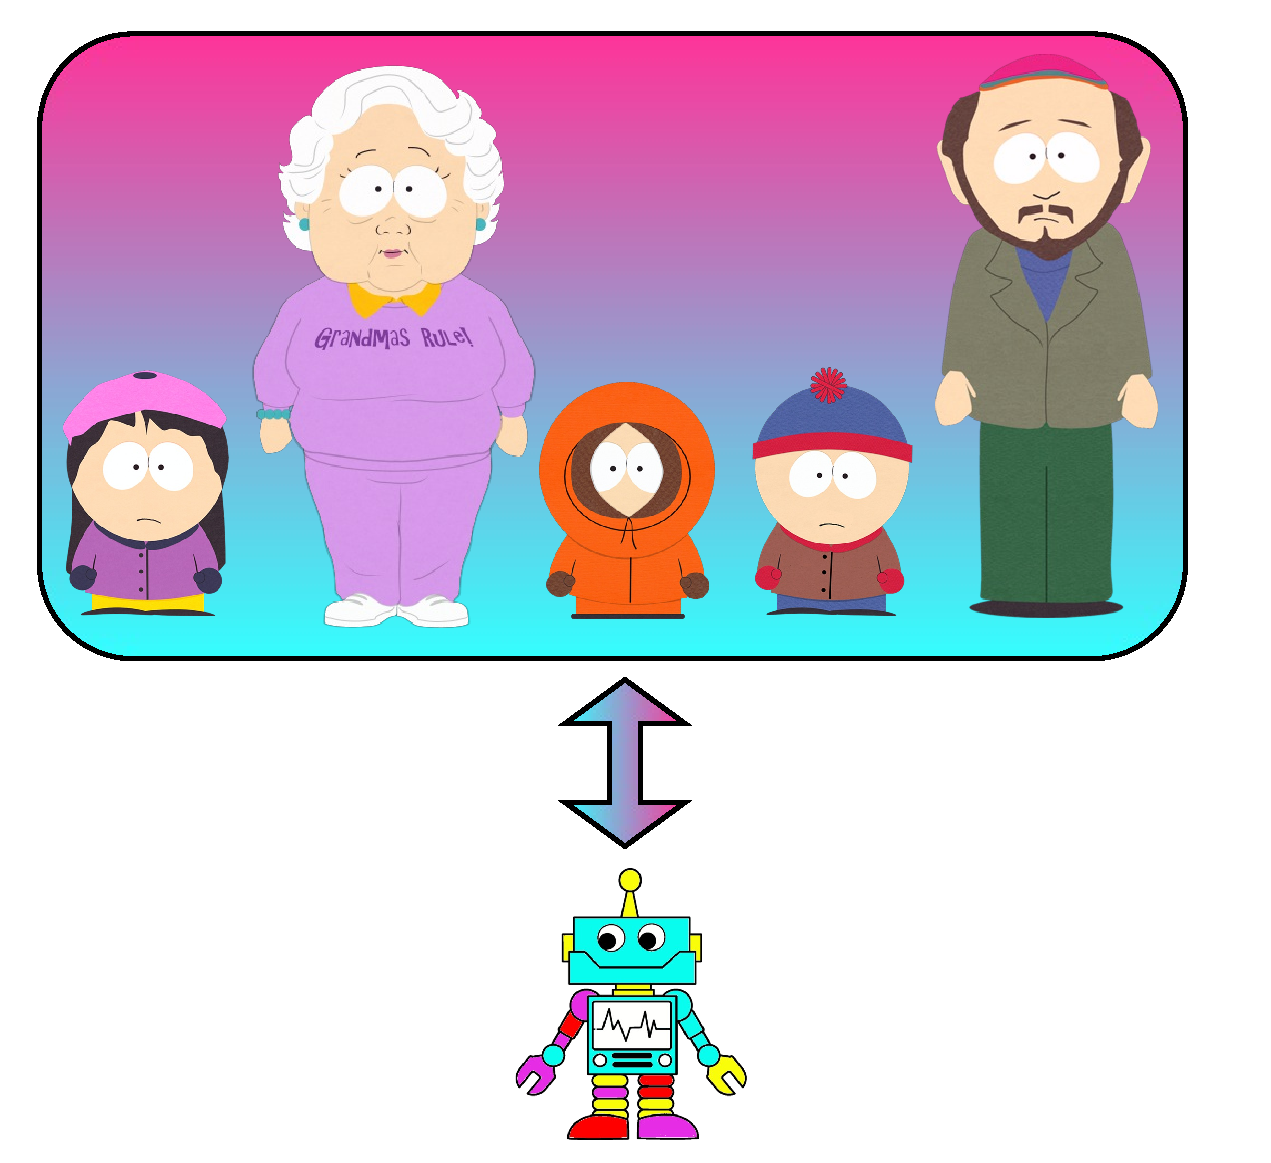
\includegraphics[width=0.6\textwidth]{img/adap0.pdf}
                % Un Anneau pour les gouverner tous
            \end{center}
        \end{figure}
    \end{frame}

    \begin{frame}{\textbf{Systèmes de dialogue} | avec adaptation}
        \begin{figure}
            \begin{center}
                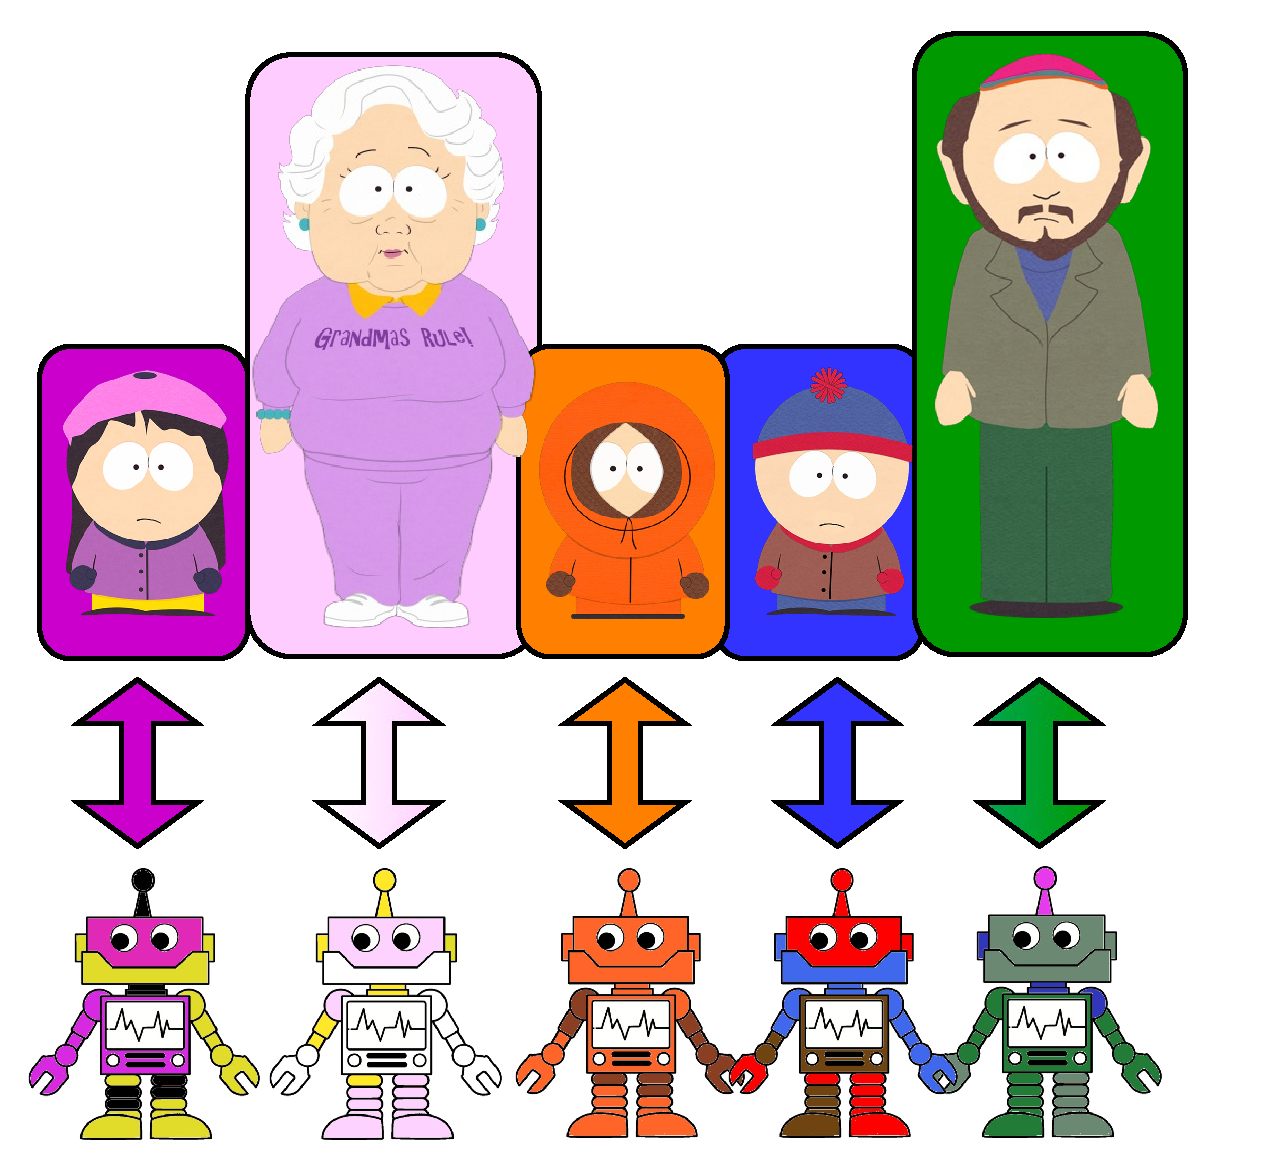
\includegraphics[width=0.6\textwidth]{img/adap1.pdf}
                % comment savoir quel système utiliser ?
            \end{center}
        \end{figure}
    \end{frame}

    \begin{frame}{Personalisation}

        % avec l'essort du smartphone/car/etc
        De plus en plus de systèmes deviennent personnels

        \begin{itemize}
            \item Assistants personnels % par définition personnels
            \item Maisons connectées % parler à l'enfant, les parents etc (les enfants sont moins succeptible de demander certain choses etc)
            \item Voitures connectées
            % handfree gps etc
        \end{itemize}

        \todo{TODO mettre deux trois images ici}

    \end{frame}

    \begin{frame}{Problématique}

        On pourrait discriminer deux types de personalisations

        \begin{itemize}
            \item Adaptation aux habitudes de la personne.
            % les rdv sont plutot le dimanche, le medecin s'appelle X, la personne habide dans un coin avec certains restaurant
            \item Adaptation au type de personne.
            % personne agée, enfant, dyslesique, culture (red good chine, red wrong europe) etc
        \end{itemize}

        %C'est surtout la deuxième problématique qui nous interesse.
        \todo{mettre en gras ou avant la deuxième problématique}

        \begin{alertblock}{Problématique}
            Comment s'adapter sans a priori? Utiliser l'apprentissage par transfert.
            % mais tout d'abord qu'est ce qu'un système de dialogue
        \end{alertblock}

    \end{frame}


    \section{Systèmes de dialogue orientées tâches}



    \subsection{Une architecture modulaire}


    \begin{frame}{L'exemple du Slot-Filling}

        Expliquer le slot filling

        Faire la transition sur comment modéliser le processus

    \end{frame}

    \foreach \n in {1,2,3,4,5,6,7}{
    \begin{frame}{Le processus (\n/7)}
        \begin{figure}
            \centering
            %%\vspace{-1.5em}
            \includegraphics[scale=0.7,page=1]{img/pipeline\n}
        \end{figure}
    \end{frame}
    }

    \foreach \n in {1,2}{
    \begin{frame}{Un problème de décision séquentielle (\n/2)}
        \begin{figure}
            \centering
            %%\vspace{-1.5em}
            \includegraphics[scale=0.55,page=1]{img/pipeline-dp\n}
        \end{figure}
    \end{frame}
    }




    \begin{frame}
        %On réduit le problème à cette échange
        \begin{figure}
            \centering
            %%\vspace{-1.5em}
            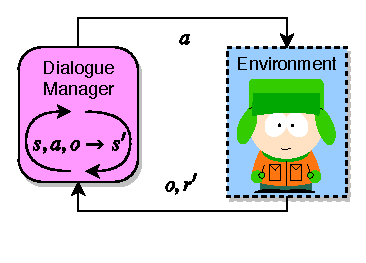
\includegraphics[scale=1.0,page=1]{../sources/dm-rl/rl-pipeline}
        \end{figure}
        \todo{dire a quoi correspond chaque etat, par rapport au slide de slot filling}

        \begin{alertblock}{}
            Comment décider l'action à choisir en fonction de l'état courant ?
        \end{alertblock}
    \end{frame}

    \subsection{Apprentissage par renforcement}
    \begin{frame}{Markov Decision Processes}

        Un MDP est un tuple $\langle{}\cS,\cA,\reward,\transition,\discountfactor\rangle{}$ où:
        \begin{itemize}
            \item  $\cS$ est l'espace des états,
            \item  $\cA$ est l'espace des actions,
            \item $\reward\in\Real^{\cS \times \cA}$ est la fonction de récompense,
            \item $\transition\in \cM(\cS)^{\cS \times \cA}$ is the transition kernel; $\cM(\cX)$ denotes the probability measure over a set $\cX$.
            \item $\discountfactor$ is the discount factor.
        \end{itemize}

    \end{frame}

    \begin{frame}{Résoudre un MDP}
        \begin{itemize}
            \item A policy $\policy\in\cM(\cA)^{\cS}$ % that maps states to actions
            \item The return $\return^{\policy} = \sum_{\indextransition=0}^\infty \discountfactor^{\indextransition} \reward(s_{\indextransition},a_{\indextransition})$% expliquer s_i et a_i
            \item Optimal policy :  $\policy^* = \argmax\limits_{\policy} \mathbb{E}_{\policy} [\return^{\policy}|s_0=s,a_0=a]\ \forall (s,a) \in \cS\times\cA$

            \item $\Q^*(s,a)=\reward(s,a) +\discountfactor \sum_{s'\in \cS}[\transition(s,a,s')\max_{a'\in \cA}\Q^*(s',a')] = \bo Q^*.$
            % It exists a unique function, denoted as $\Q^*$, that verifies the Bellman Optimality equation:

            \item $\optimalpolicy(s) \in \argmax\limits_{a\in \cA} \Q^*(s,a)$ is optimal.
        \end{itemize}


    \end{frame}

    \begin{frame}{Algoritmes}

        \begin{block}{Value-Iteration}
            \begin{itemize}
                \item $Q \leftarrow \mathbf{0}$
                \item $Q(s,a) \leftarrow \bo Q(s,a)\ \forall (s,a)$ until convergence
                \item Return $\pi(s) = \argmax\limits_{a} Q(s,a)$
            \end{itemize}
        \end{block}

        \begin{alertblock}{}
            \begin{itemize}
                \item How to compute $\bo Q$ if $\transition$ and $\reward$ unknown?
                \item How to compute $Q \forall (s,a) \in \cS\times\cA$ if $S$ is continous or very large ?
            \end{itemize}

        \end{alertblock}

        \begin{block}{Fitted-Q}
            \begin{itemize}
                \item $Q \leftarrow \mathbf{0}$
                \item $Q \leftarrow \Gamma(\{s_{\indextransition},a_{\indextransition}\}_{{\indextransition}\in \T},\{r'_{\indextransition} + \discountfactor  \max_{a'\in\cA} \Q(s'_i,a')\}_{{\indextransition} \in \T})$
                \item Return $\pi(s) = \argmax\limits_{a} Q(s,a)$
            \end{itemize}
        \end{block}


    \end{frame}

    \begin{frame}{Comment amasser des transitions?}

        Parler du online, epsilon greedy

        \todo{faire un schéma avec un robot, les samples, + FITTEDQ}

        -> unknown env we need sample, if we don't know the user, we don't have samples -> transfer learning

    \end{frame}

    \subsection{Apprentissage par Transfert}
    \begin{frame}{Pourquoi transférer ?}

        \begin{figure}
            \begin{center}
                \subfloat[jumpstart performance]{
                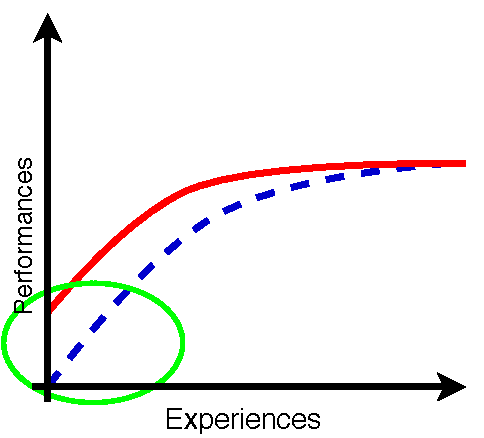
\includegraphics[width=0.33\textwidth]{../sources/dm-tl/objectives-jumpstart}
                \label{fig:objectives-jumpstart}
                }
                \subfloat[Learning performance]{
                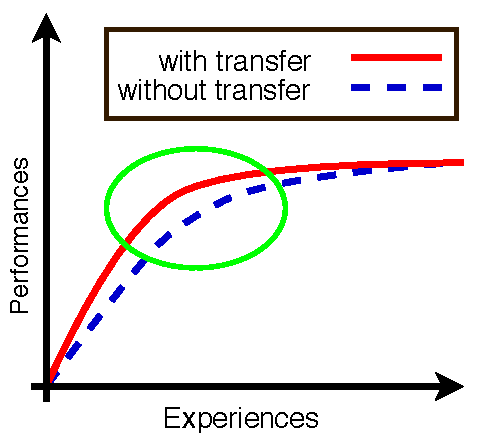
\includegraphics[width=0.33\textwidth]{../sources/dm-tl/objectives-learn}
                \label{fig:objectives-learn}
                }
                \subfloat[Asymptotic performance]{
                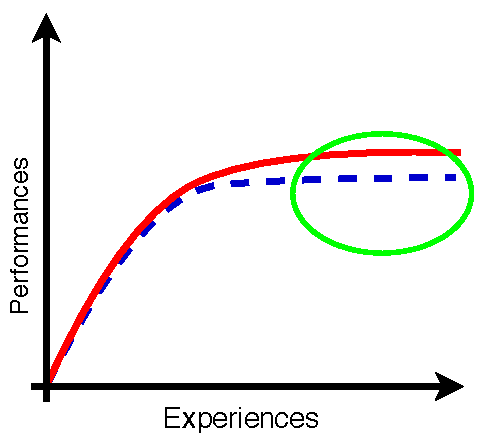
\includegraphics[width=0.33\textwidth]{../sources/dm-tl/objectives-asymptote}
                \label{fig:objectives-asymptote}
                }
                \caption{Objectives of Transfert Learning~\parencite{langley2006,LazaricSurvey}}
                \label{fig:objectives}
            \end{center}
        \end{figure}

    \end{frame}

    \begin{frame}{Les différentes formes de transfert}


        \begin{itemize}
            \item Policy
            \begin{itemize}
                \item XXX2012 etc (cité ceux lié au dialogue)
            \end{itemize}
            \item  etc
        \end{itemize}

    \end{frame}

    \begin{frame}{Contributions}

        %On va explorer
        Deux directions, toutes deux exploitant l'apprentissage par transfert.

        \begin{itemize}
            \item Approche classique, avec l'utilisation d'outils existants et leur mise à l'echelle.
            \item Approche plus conservatrice, en mettant en avant la notion de risque dans la conversation.
        \end{itemize}


    \end{frame}

    \section{Passage à l'échelle de l'apprentissage par transfert}

    \subsection{Un processus complet pour l'adaptation à l'utilisateur}



    \foreach \n in {0,1,2,3,4,5,6,7,8,9,10,11,13,14}{
    \begin{frame}{Le processus}
        \todo{but what if the system database grow ? bandit useless}
        \begin{figure}
            \begin{center}
                \includegraphics[width=0.75\textwidth]{img/dataflowRobot\n.pdf}
            \end{center}
        \end{figure}
    \end{frame}
    }

    \begin{frame}{\textbf{Sources election} | \textsc{PD-distance}}
        \begin{figure}
            \begin{center}
                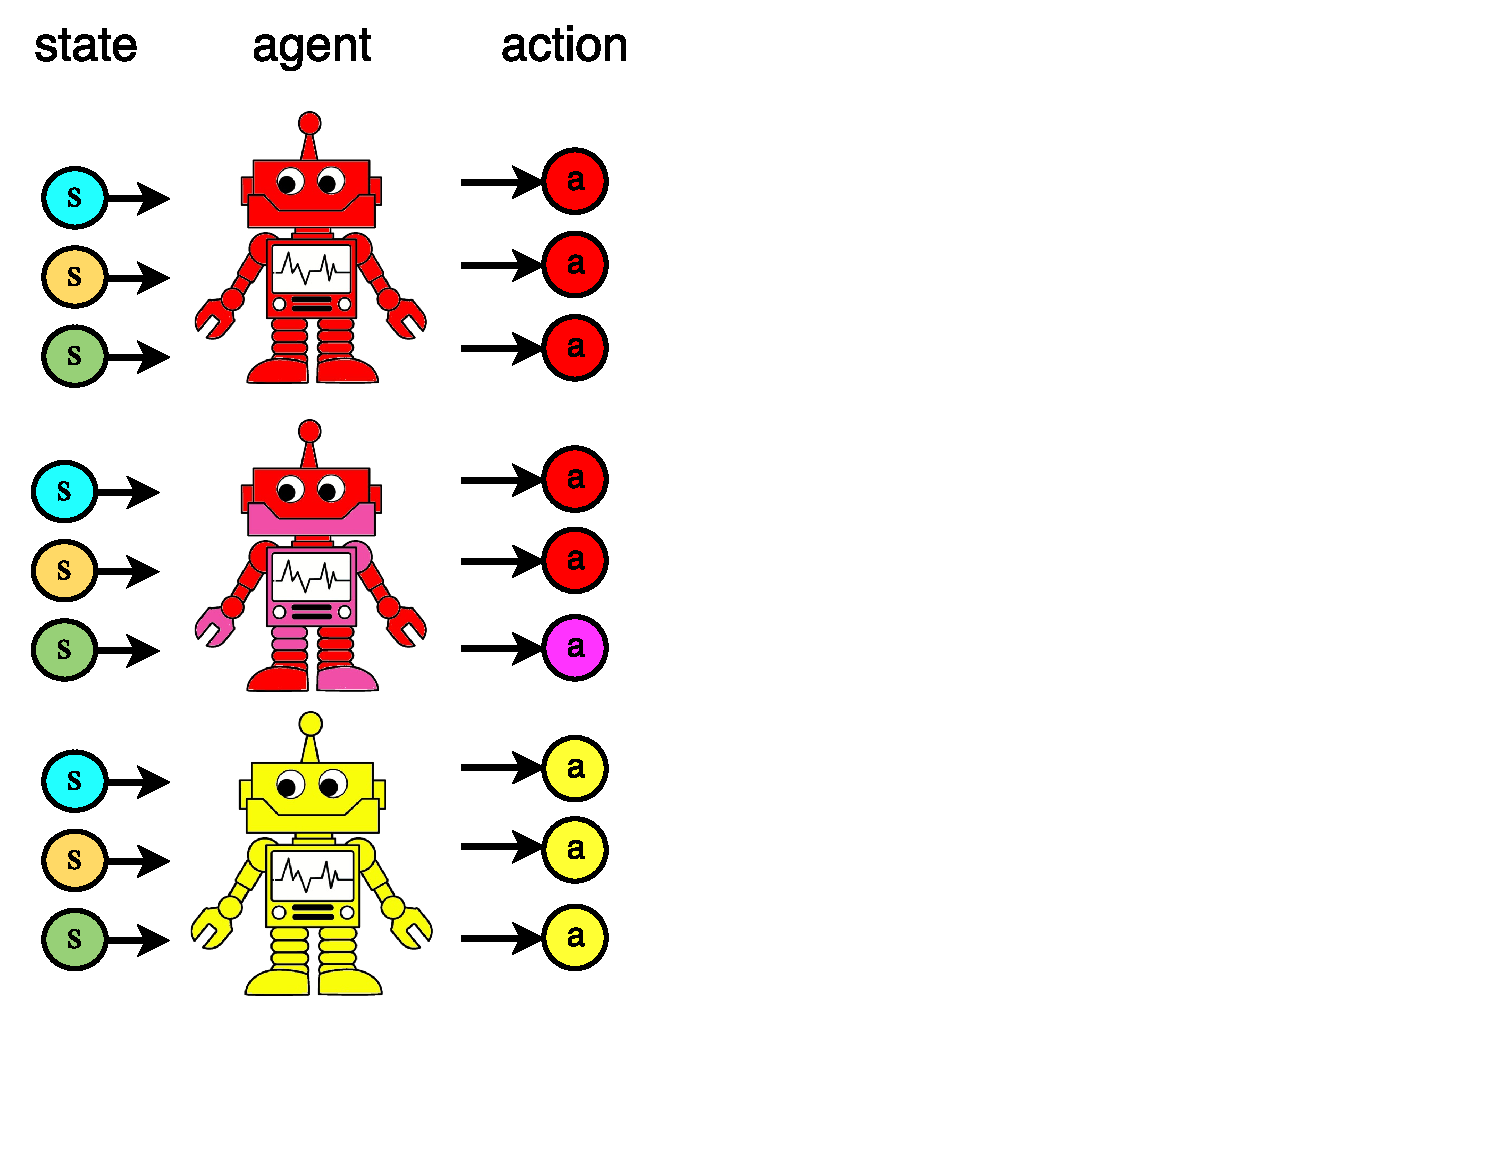
\includegraphics[width=1.0\textwidth]{img/pddistance0.pdf}
            \end{center}
        \end{figure}
    \end{frame}

    \begin{frame}{\textbf{Sources election} | \textsc{PD-distance}}
        \begin{figure}
            \begin{center}
                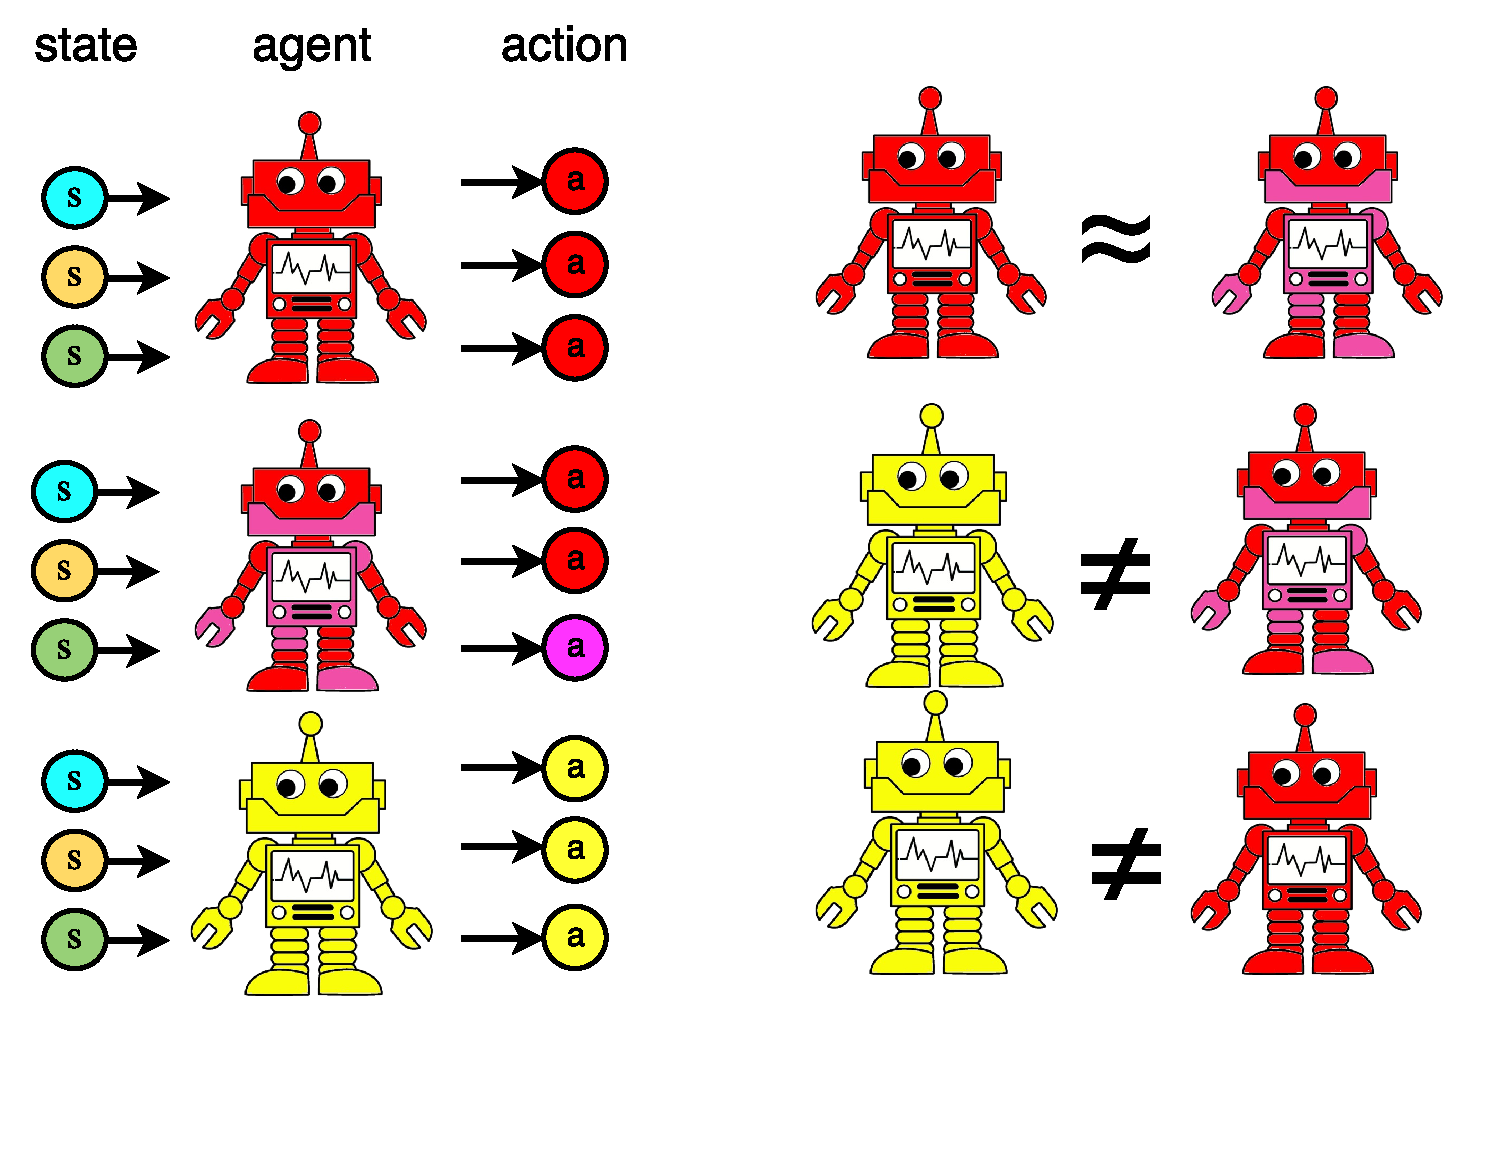
\includegraphics[width=1.0\textwidth]{img/pddistance.pdf}
            \end{center}
        \end{figure}
    \end{frame}
    \foreach \n in {0,1,2,3,4}{
    \begin{frame}{\textbf{Sources election} | \textsc{PD-distance} and euclidian norm}
        \begin{figure}
            \begin{center}
                \includegraphics[width=1.0\textwidth]{img/euclide\n.pdf}
            \end{center}
        \end{figure}
    \end{frame}
    }

    \begin{frame}{\textbf{Sources election} | \textsc{K-means}}
        \begin{figure}
            \begin{center}
                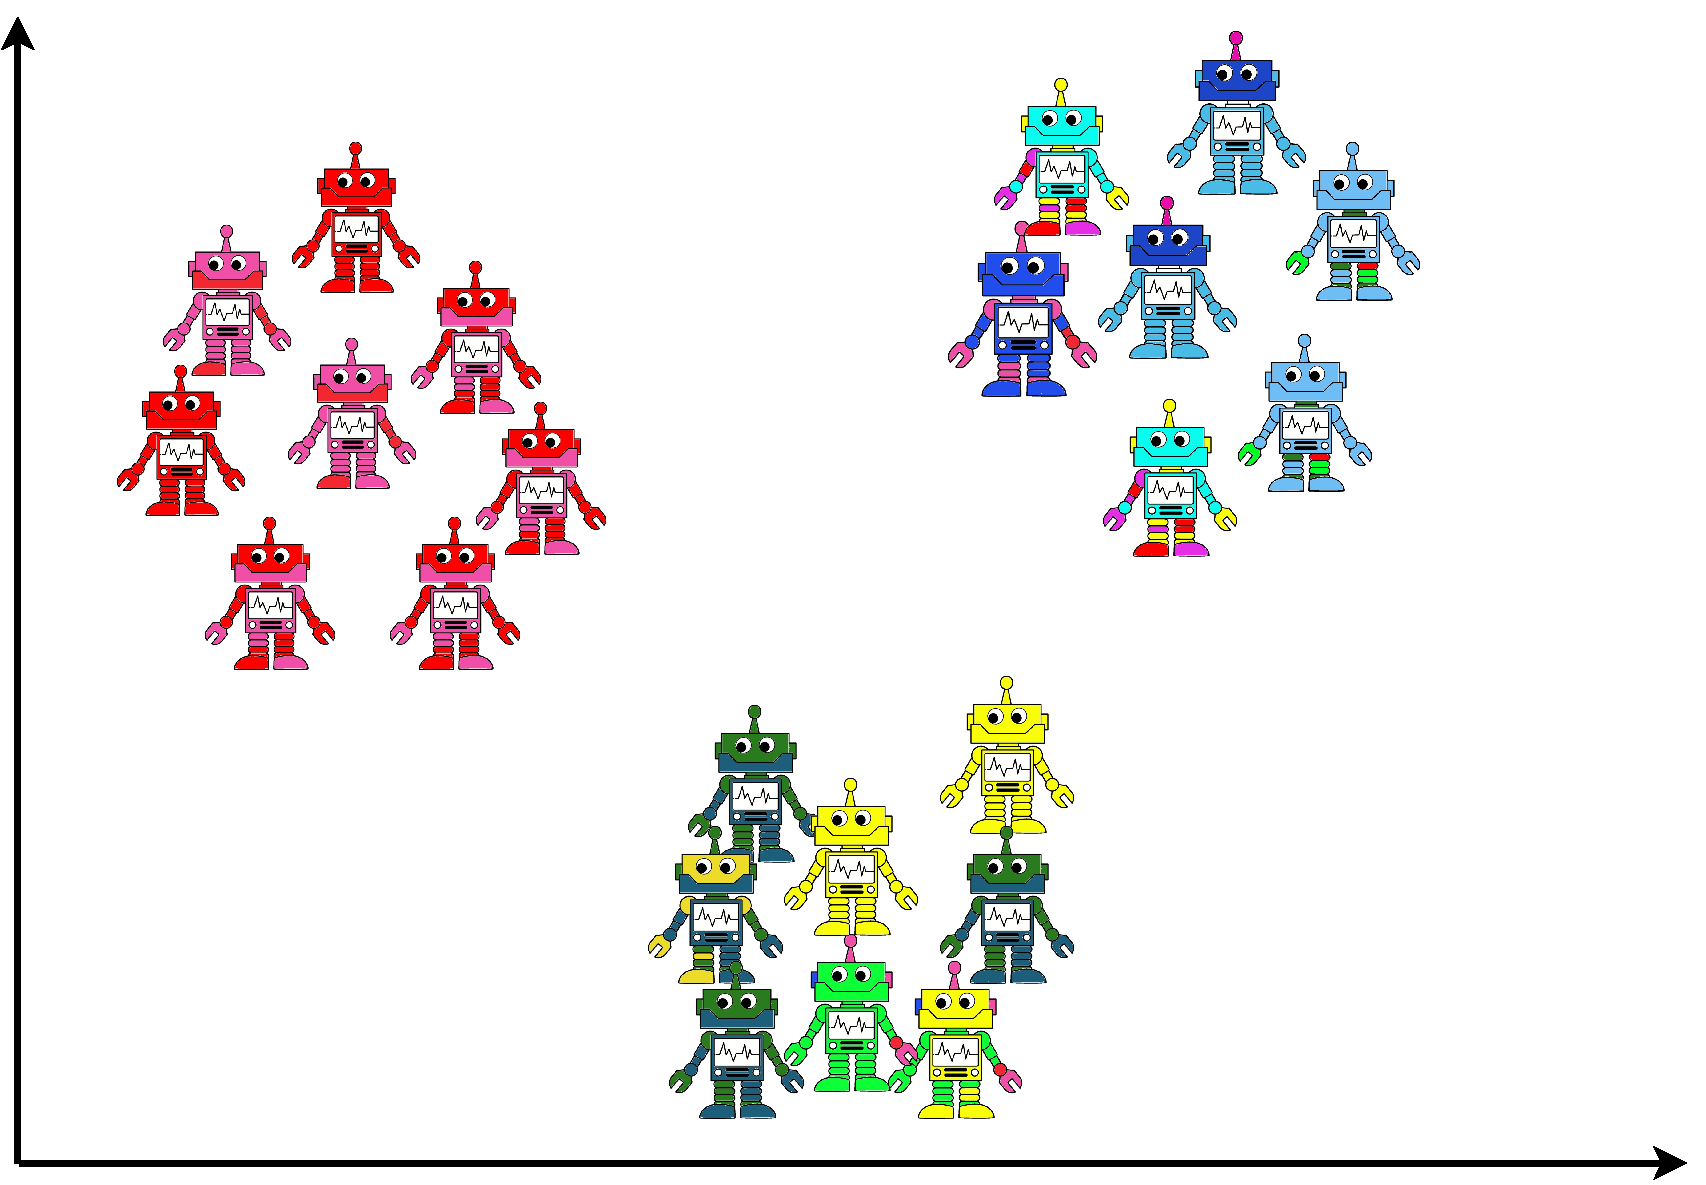
\includegraphics[width=0.85\textwidth]{img/clustering.pdf}
            \end{center}
        \end{figure}
    \end{frame}

    \foreach \n in {0}{
    \begin{frame}{\textbf{Sources election} | \textsc{K-means}}
        \begin{figure}
            \begin{center}
                \includegraphics[width=0.85\textwidth]{img/kmeans\n.pdf}
            \end{center}
        \end{figure}
    \end{frame}
    }
    \begin{frame}{\textbf{Sources election} | \textsc{K-medoids}}
        \begin{figure}
            \begin{center}
                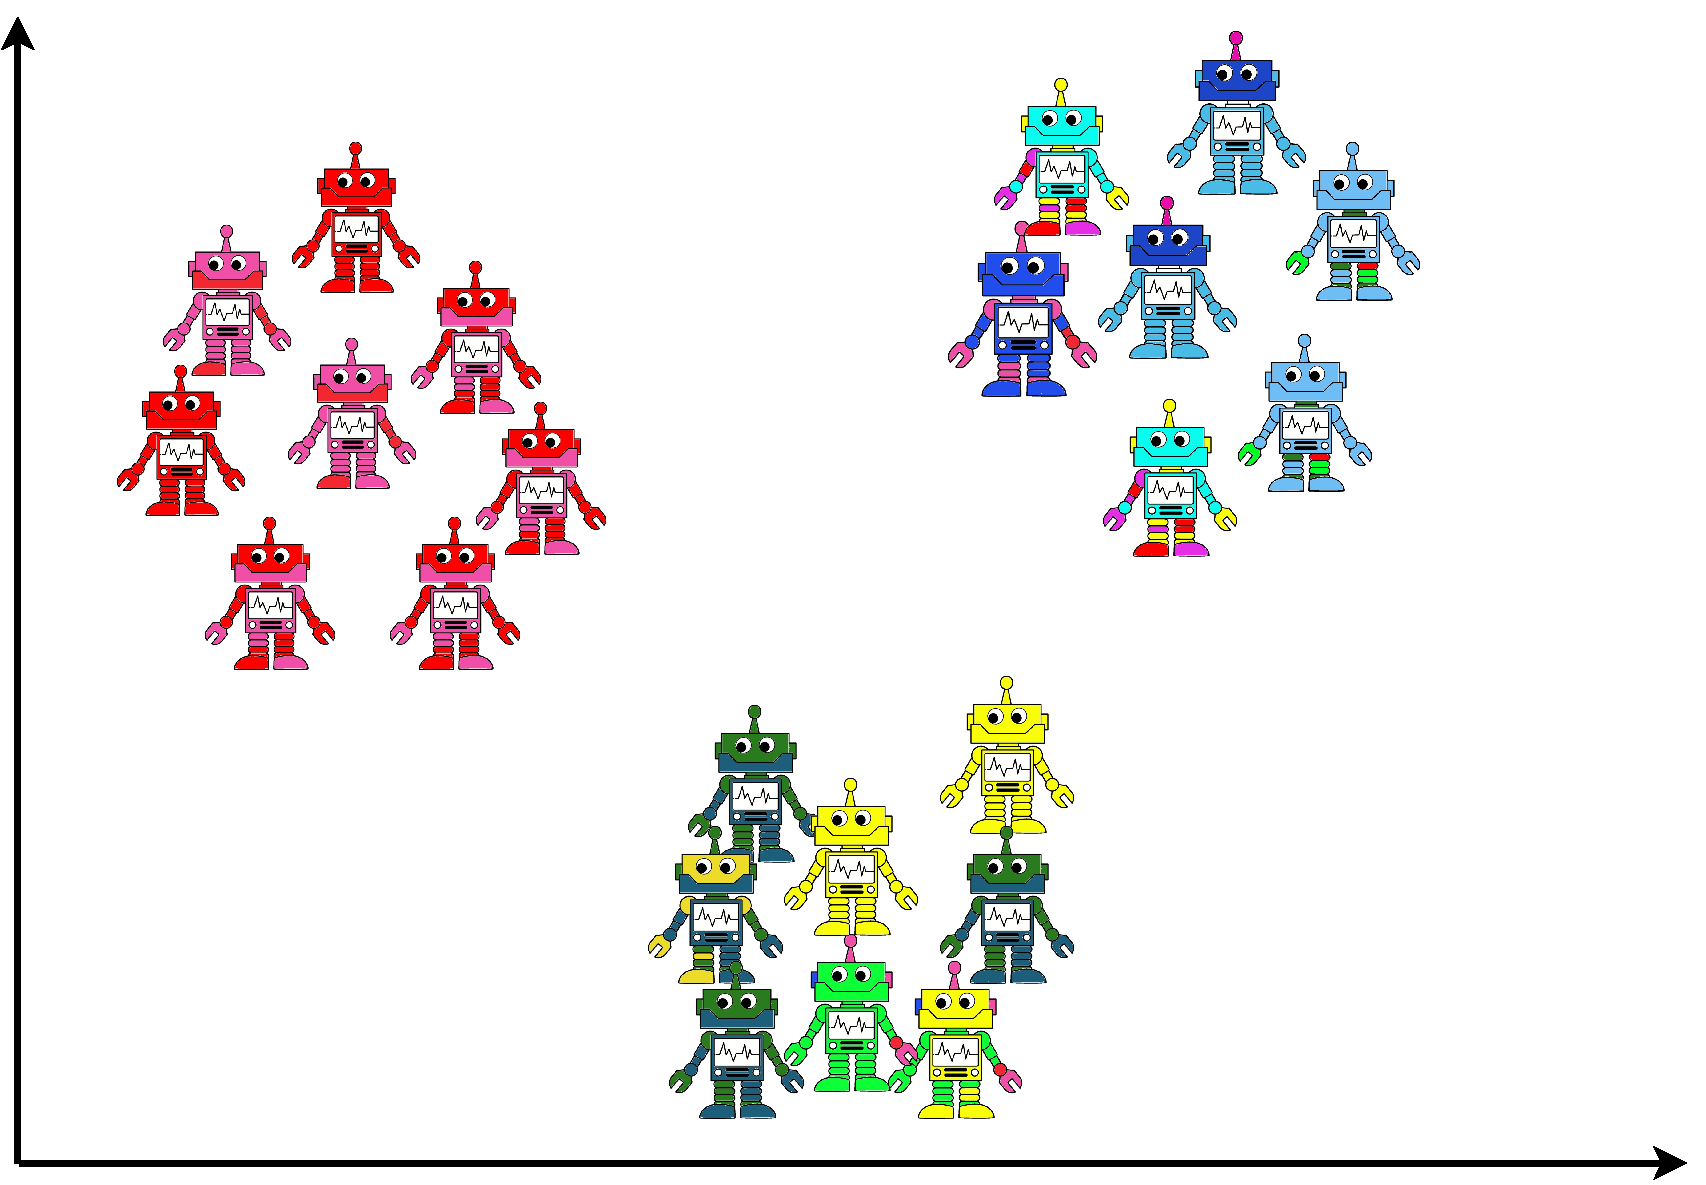
\includegraphics[width=0.85\textwidth]{img/clustering.pdf}
            \end{center}
        \end{figure}
    \end{frame}

    \begin{frame}{\textbf{Sources election} | \textsc{K-medoids}}
        \begin{figure}
            \begin{center}
                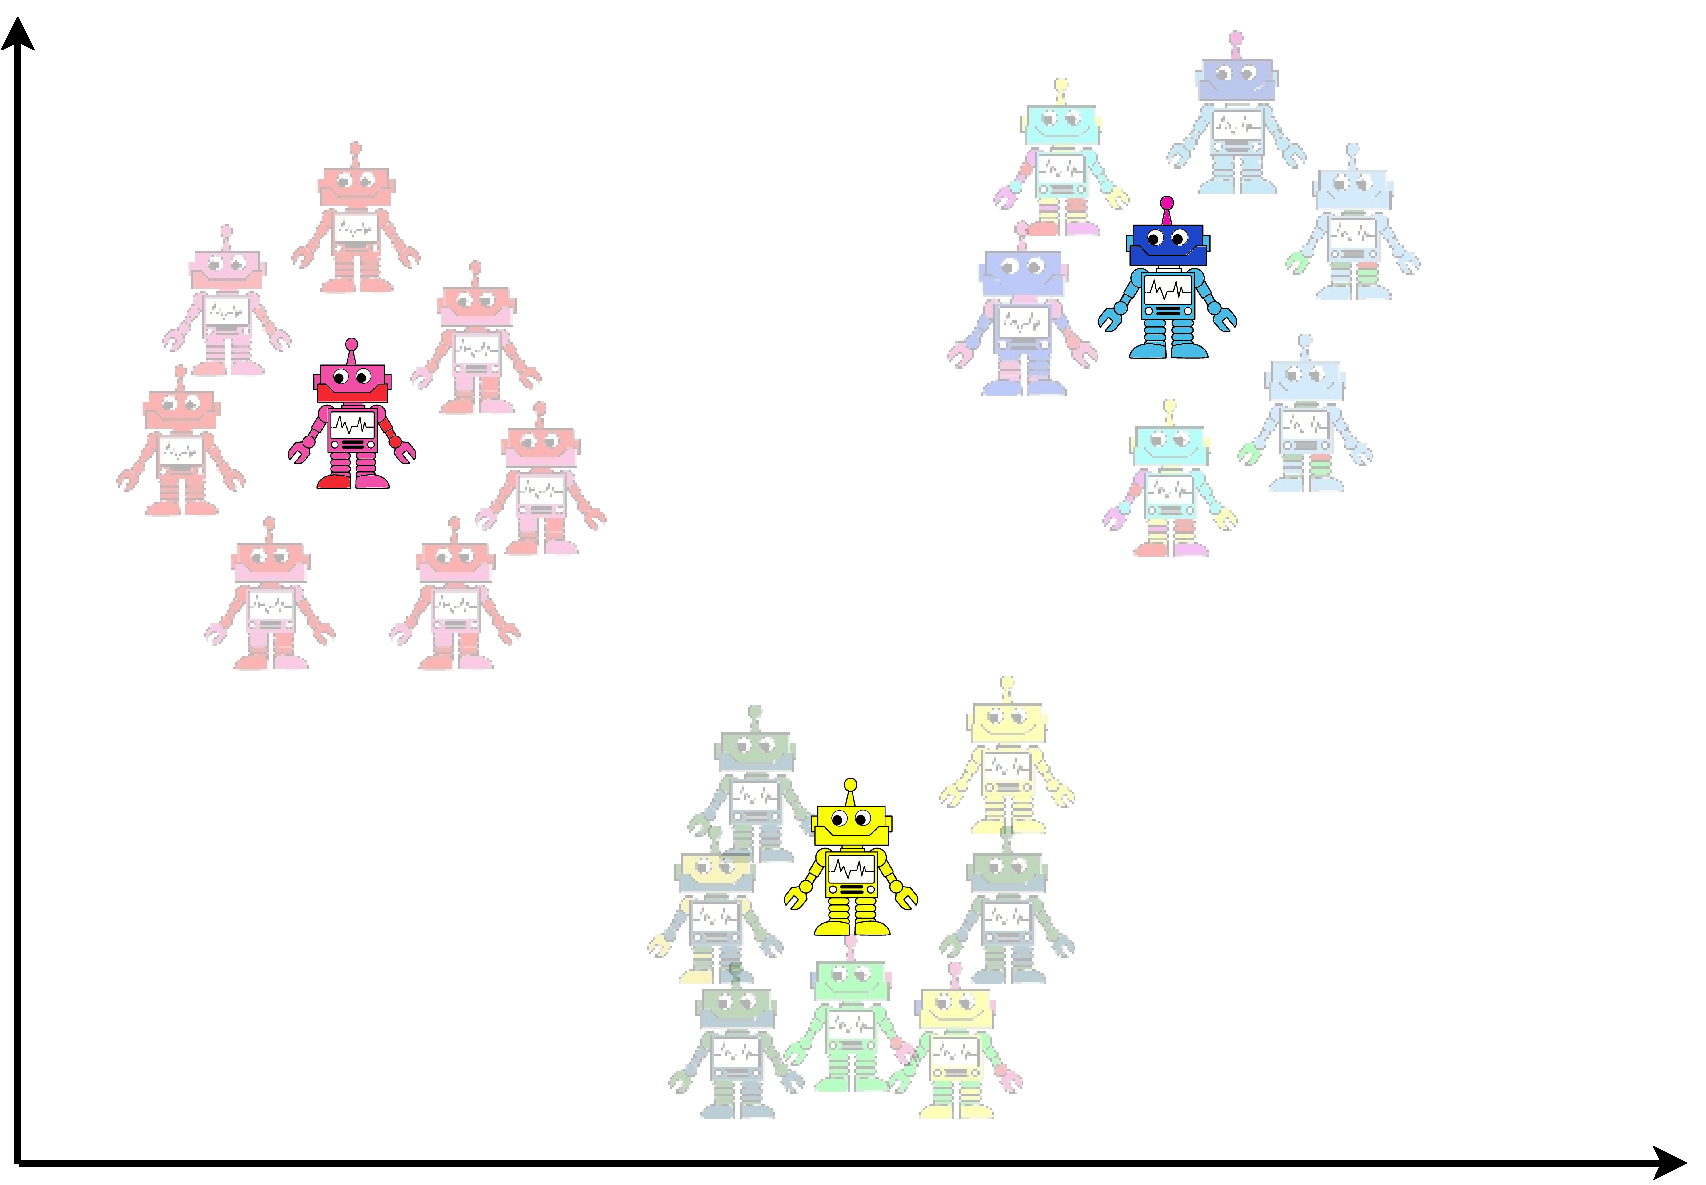
\includegraphics[width=0.85\textwidth]{img/kmedoids.pdf}
            \end{center}
        \end{figure}
    \end{frame}

    \begin{frame}{\textbf{Adaptation experiments} | simulated users}
        \todo{show dialogue lenghts}
        \begin{figure}
            \captionsetup[subfigure]{labelformat=empty}
            \begin{center}
                \subfloat[Overall score ]{
                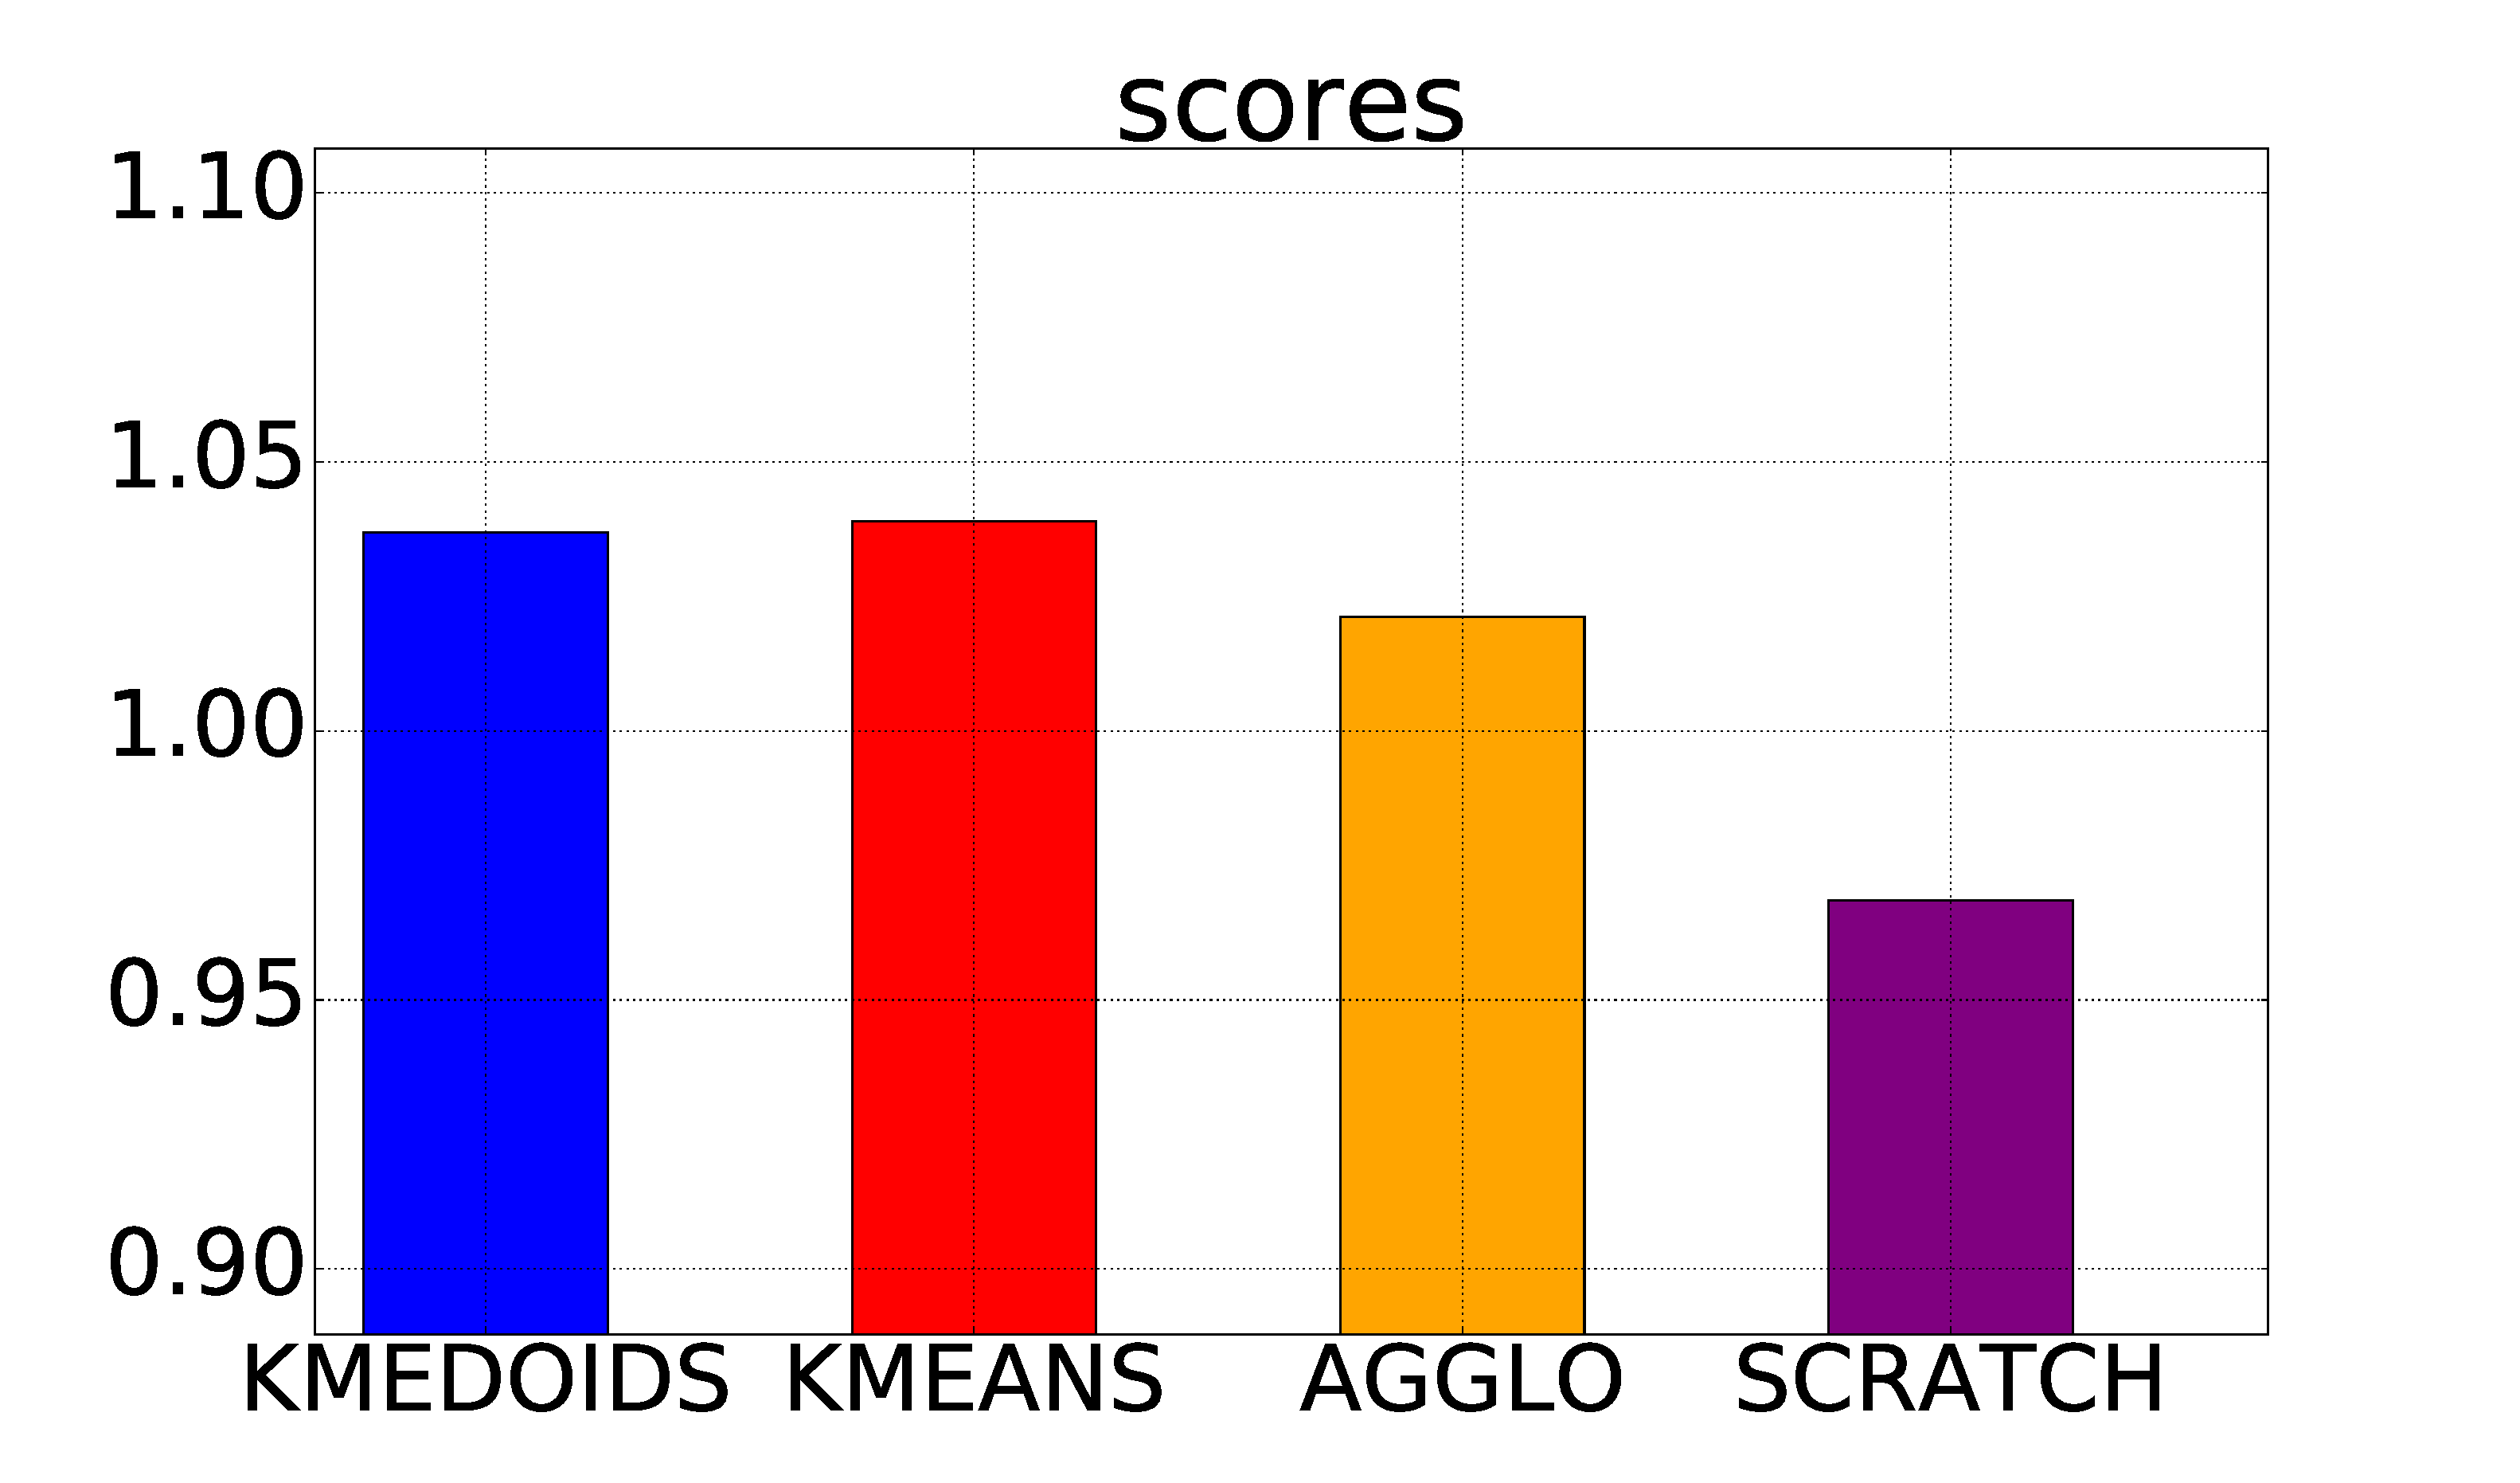
\includegraphics[width=0.5\textwidth]{img/handcraftedScores.pdf}
                }
                \subfloat[Task completion]{
                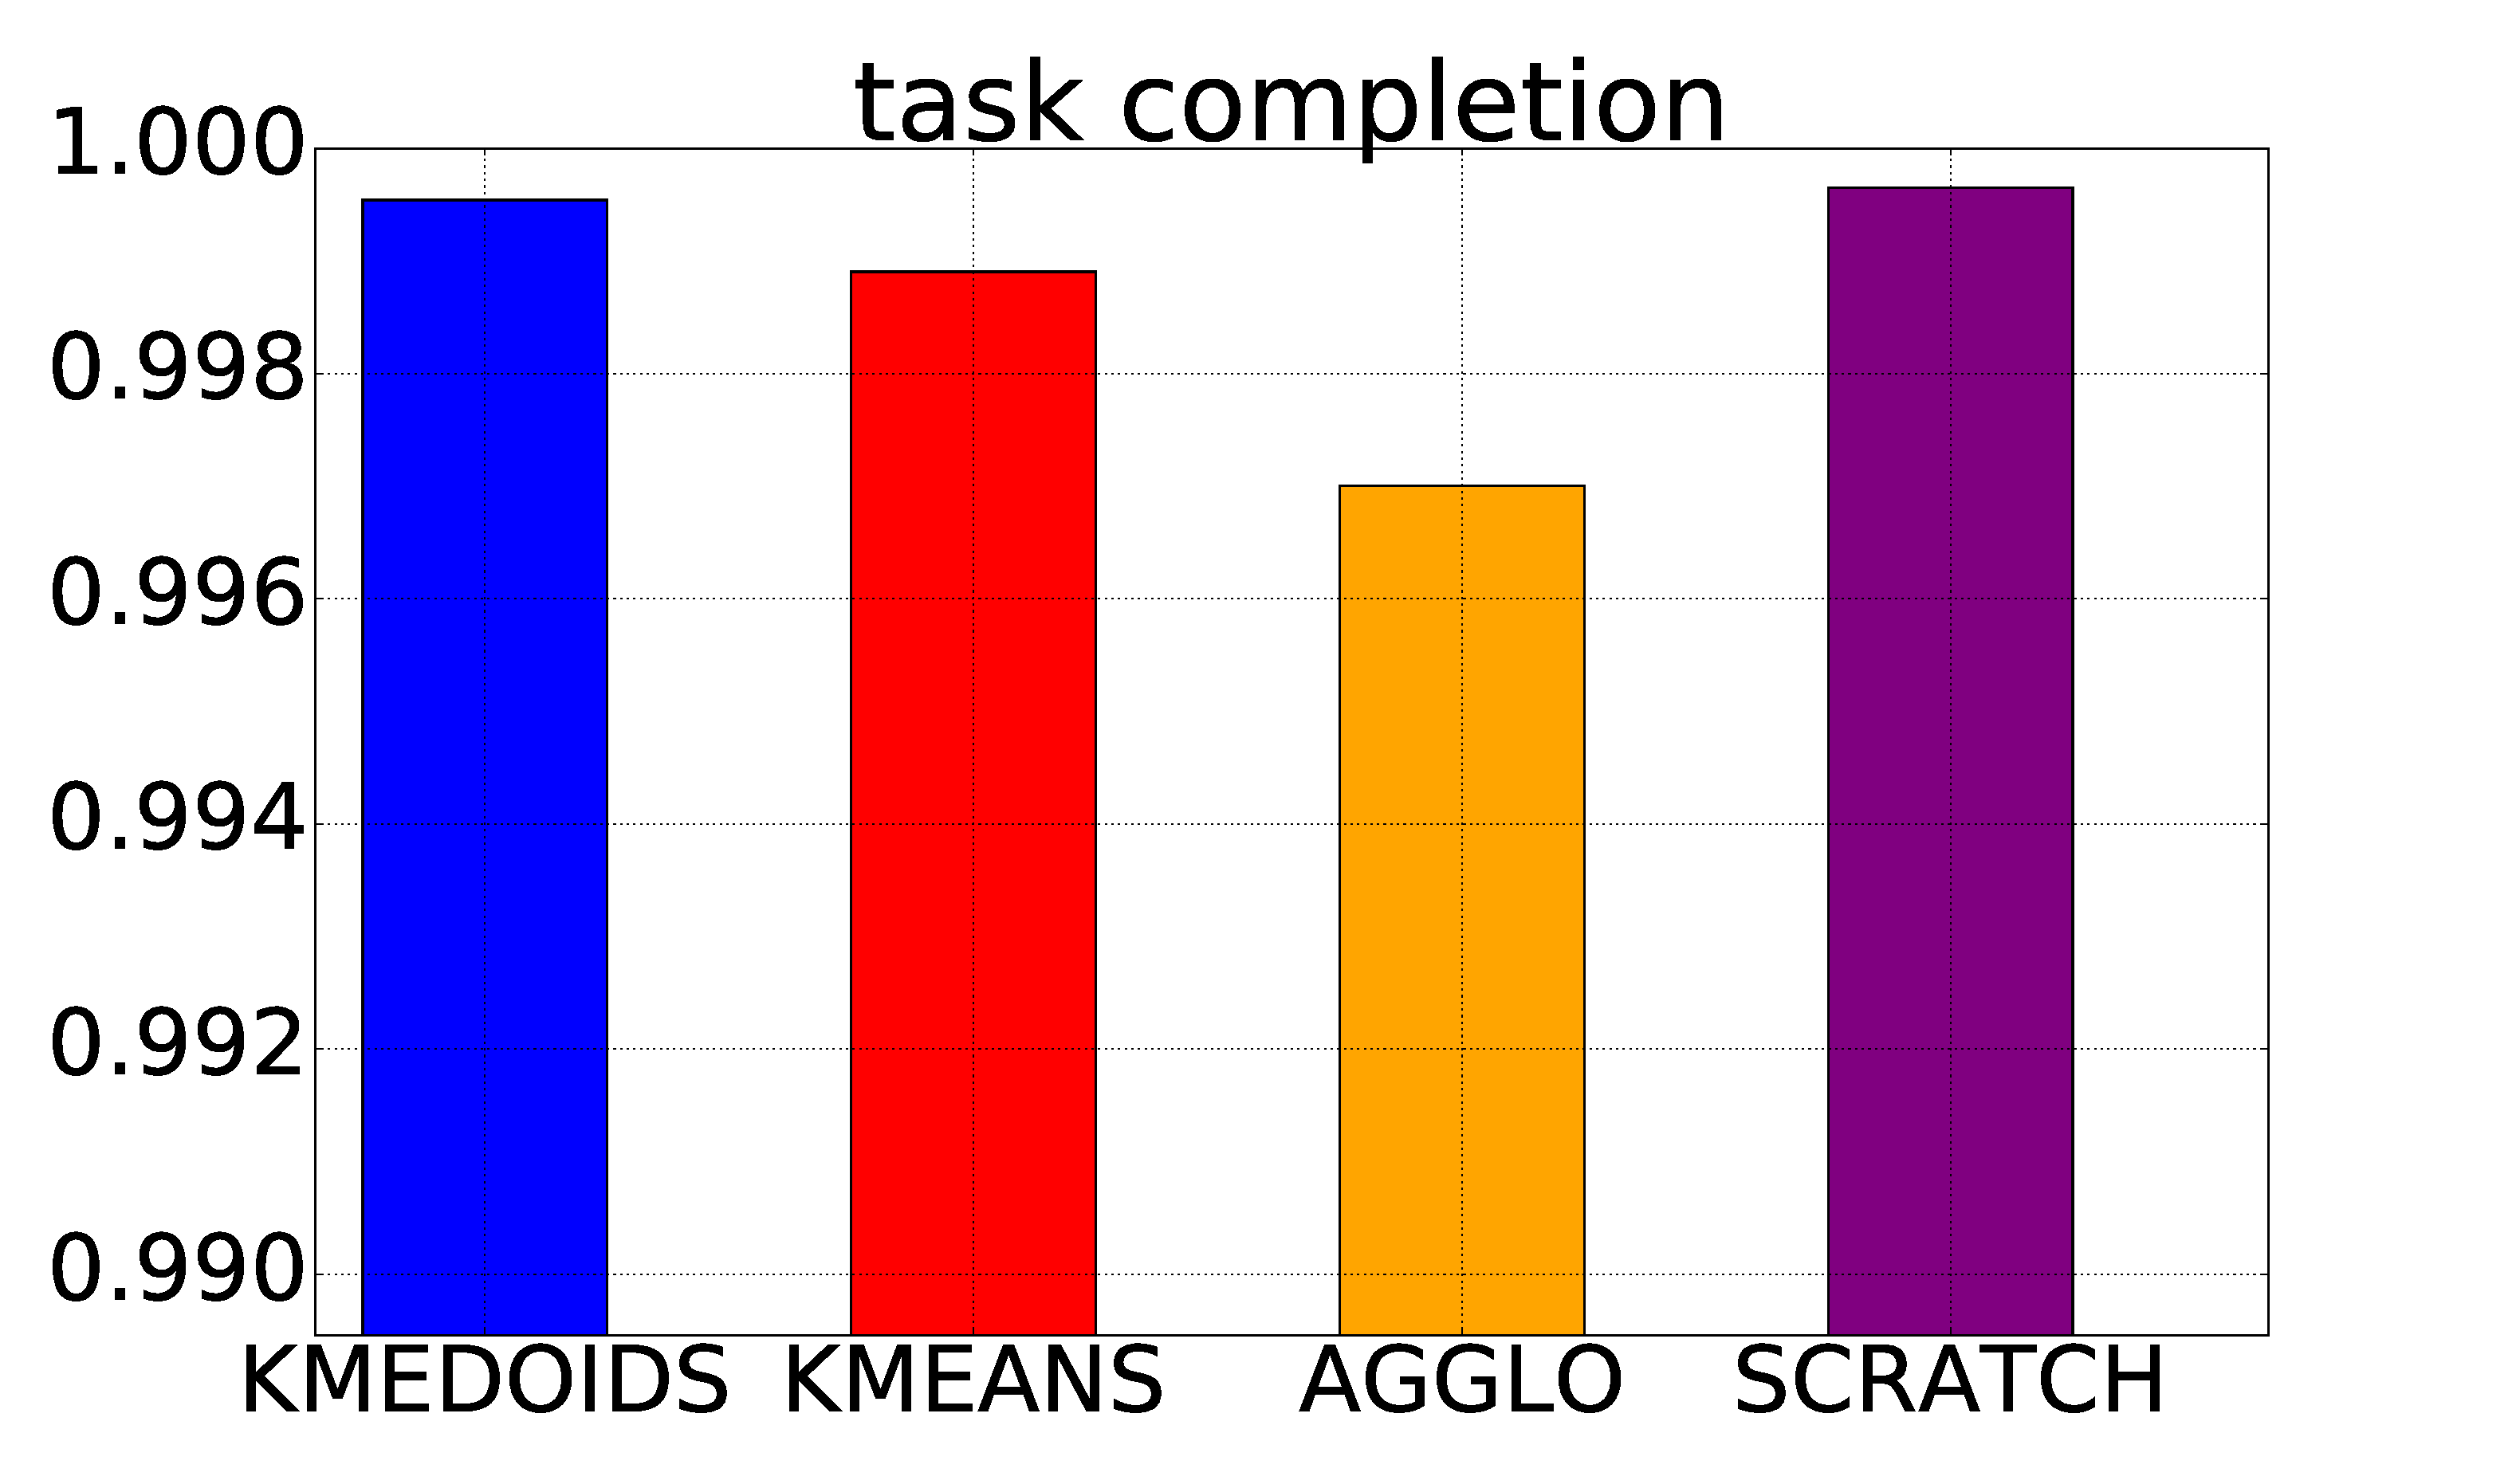
\includegraphics[width=0.5\textwidth]{img/handcraftedTC.pdf}
                }
            \end{center}
        \end{figure}
    \end{frame}

    \begin{frame}{\textbf{Adaptation experiments} | human-model users}
        \begin{figure}
            \captionsetup[subfigure]{labelformat=empty}
            \begin{center}
                \subfloat[Overall score ]{
                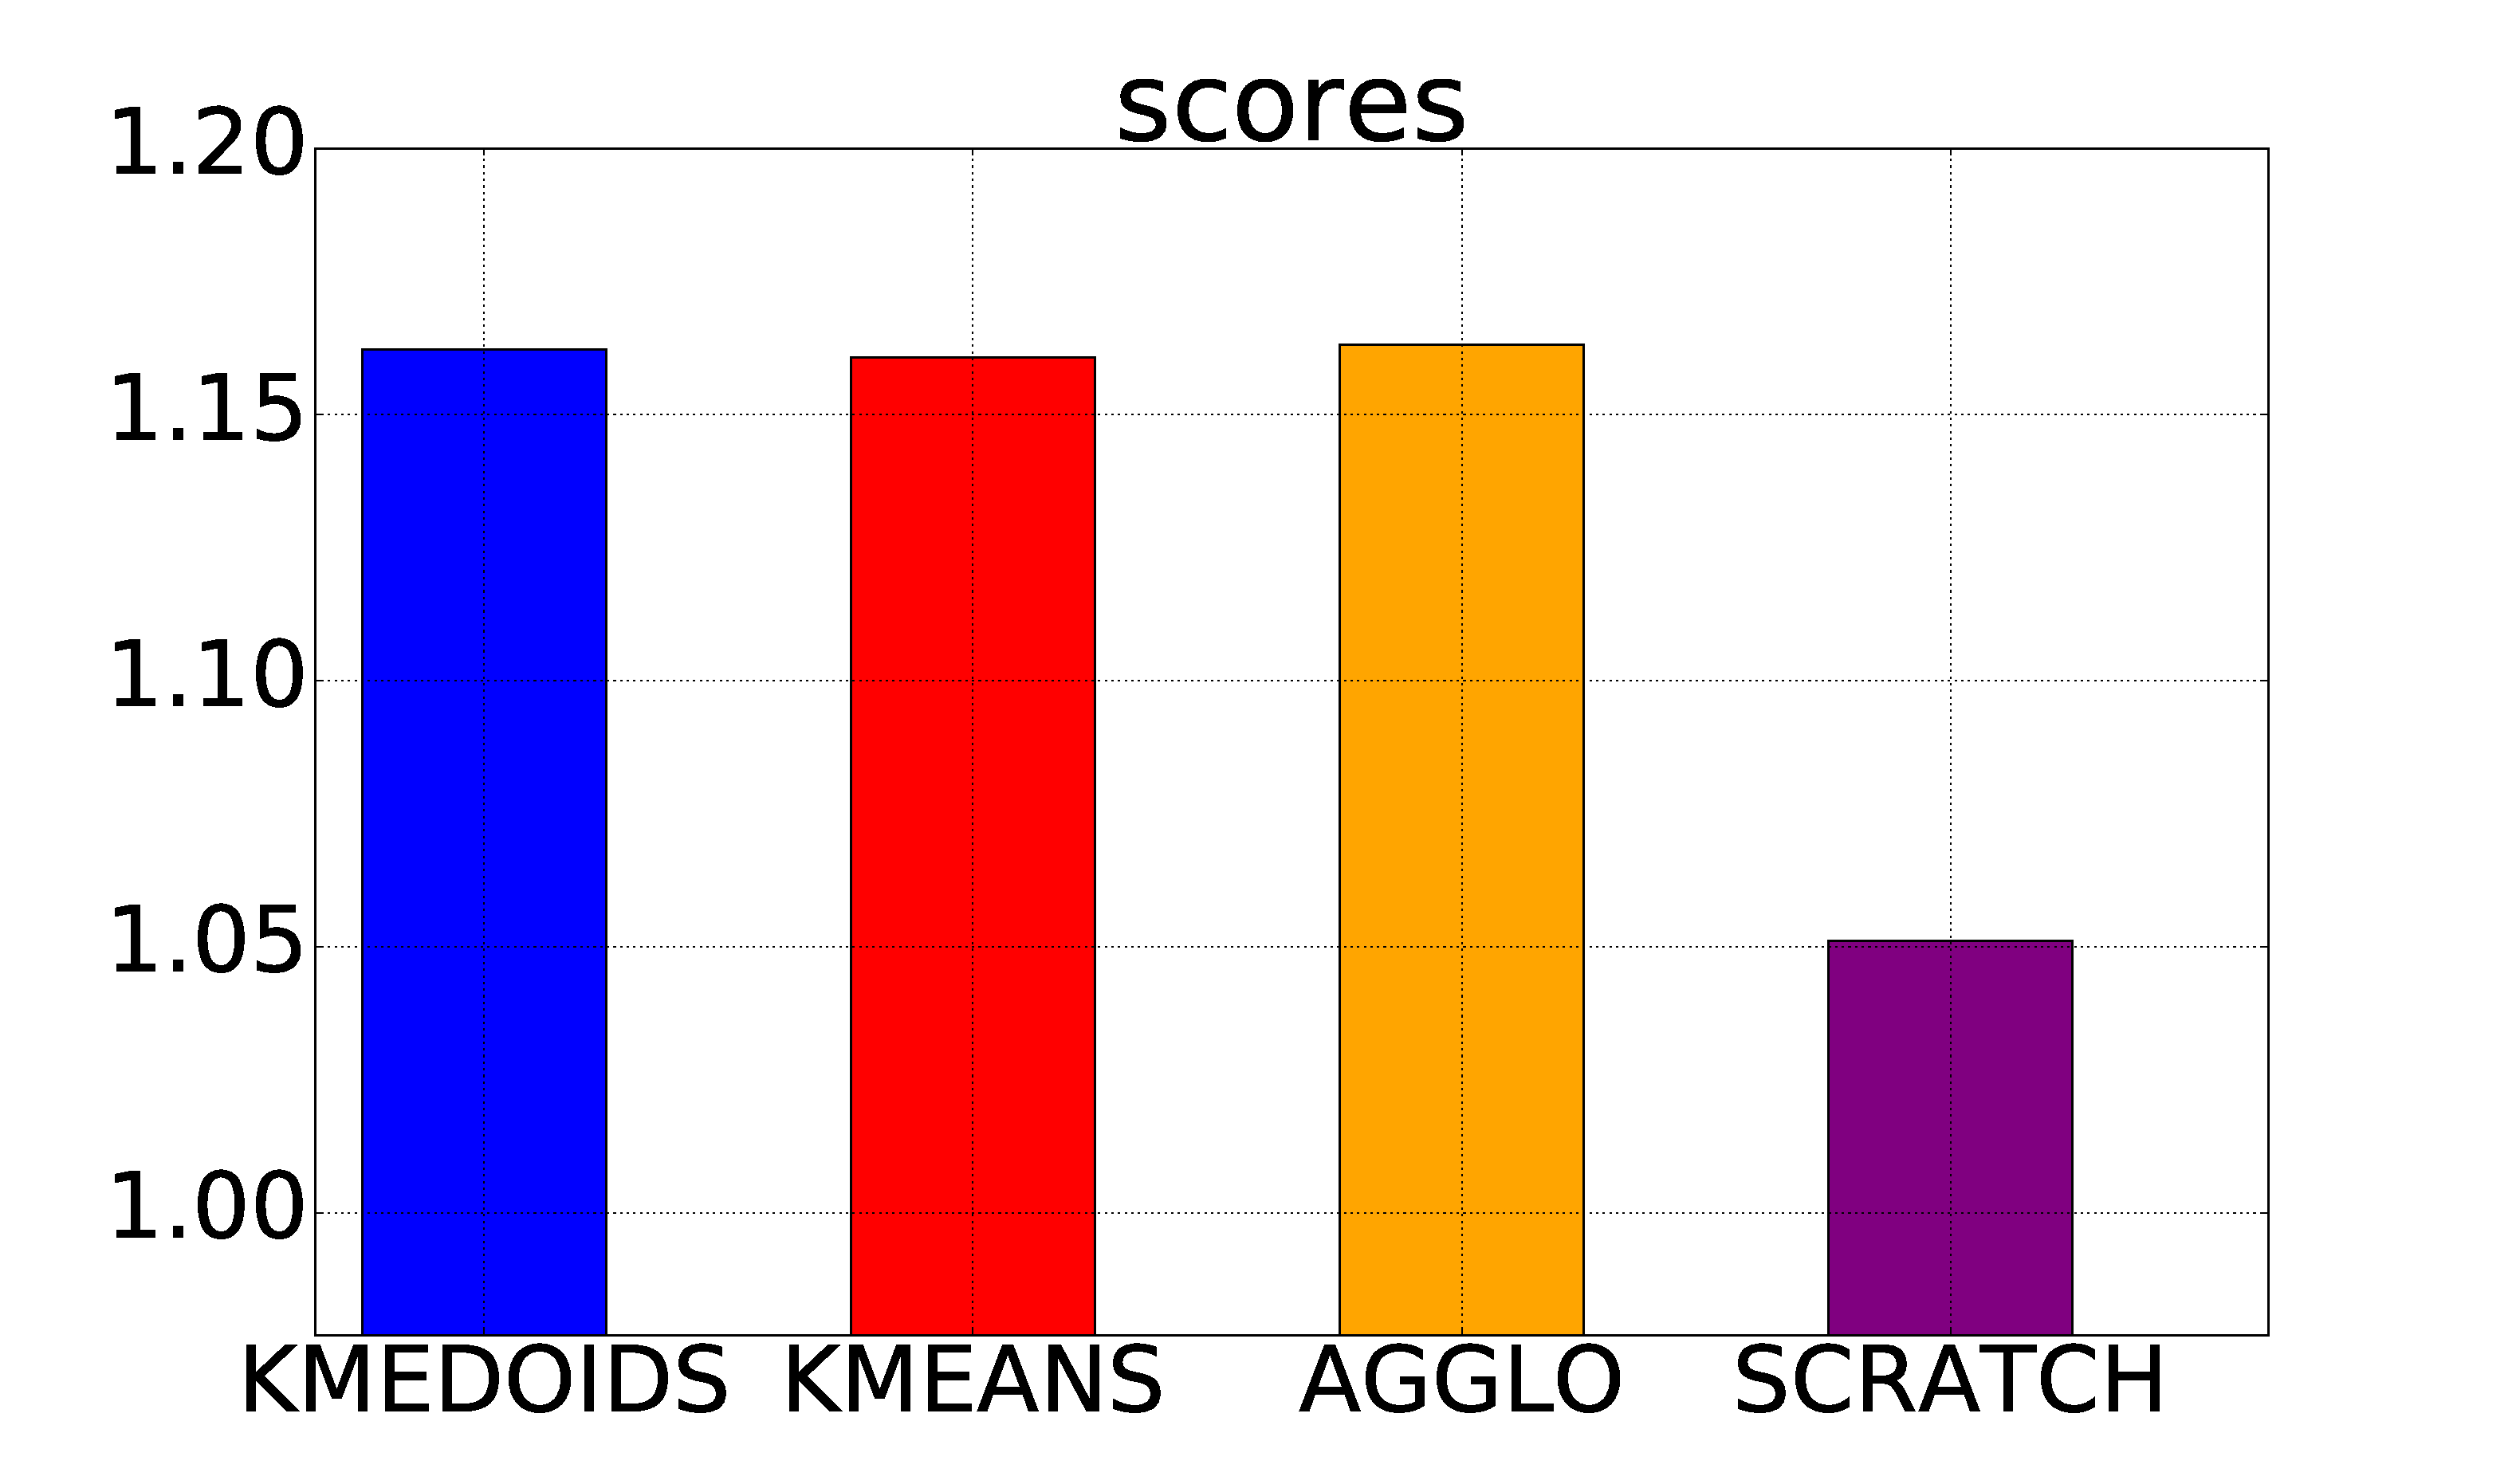
\includegraphics[width=0.5\textwidth]{img/humanScores.pdf}
                }
                \subfloat[Task completion]{
                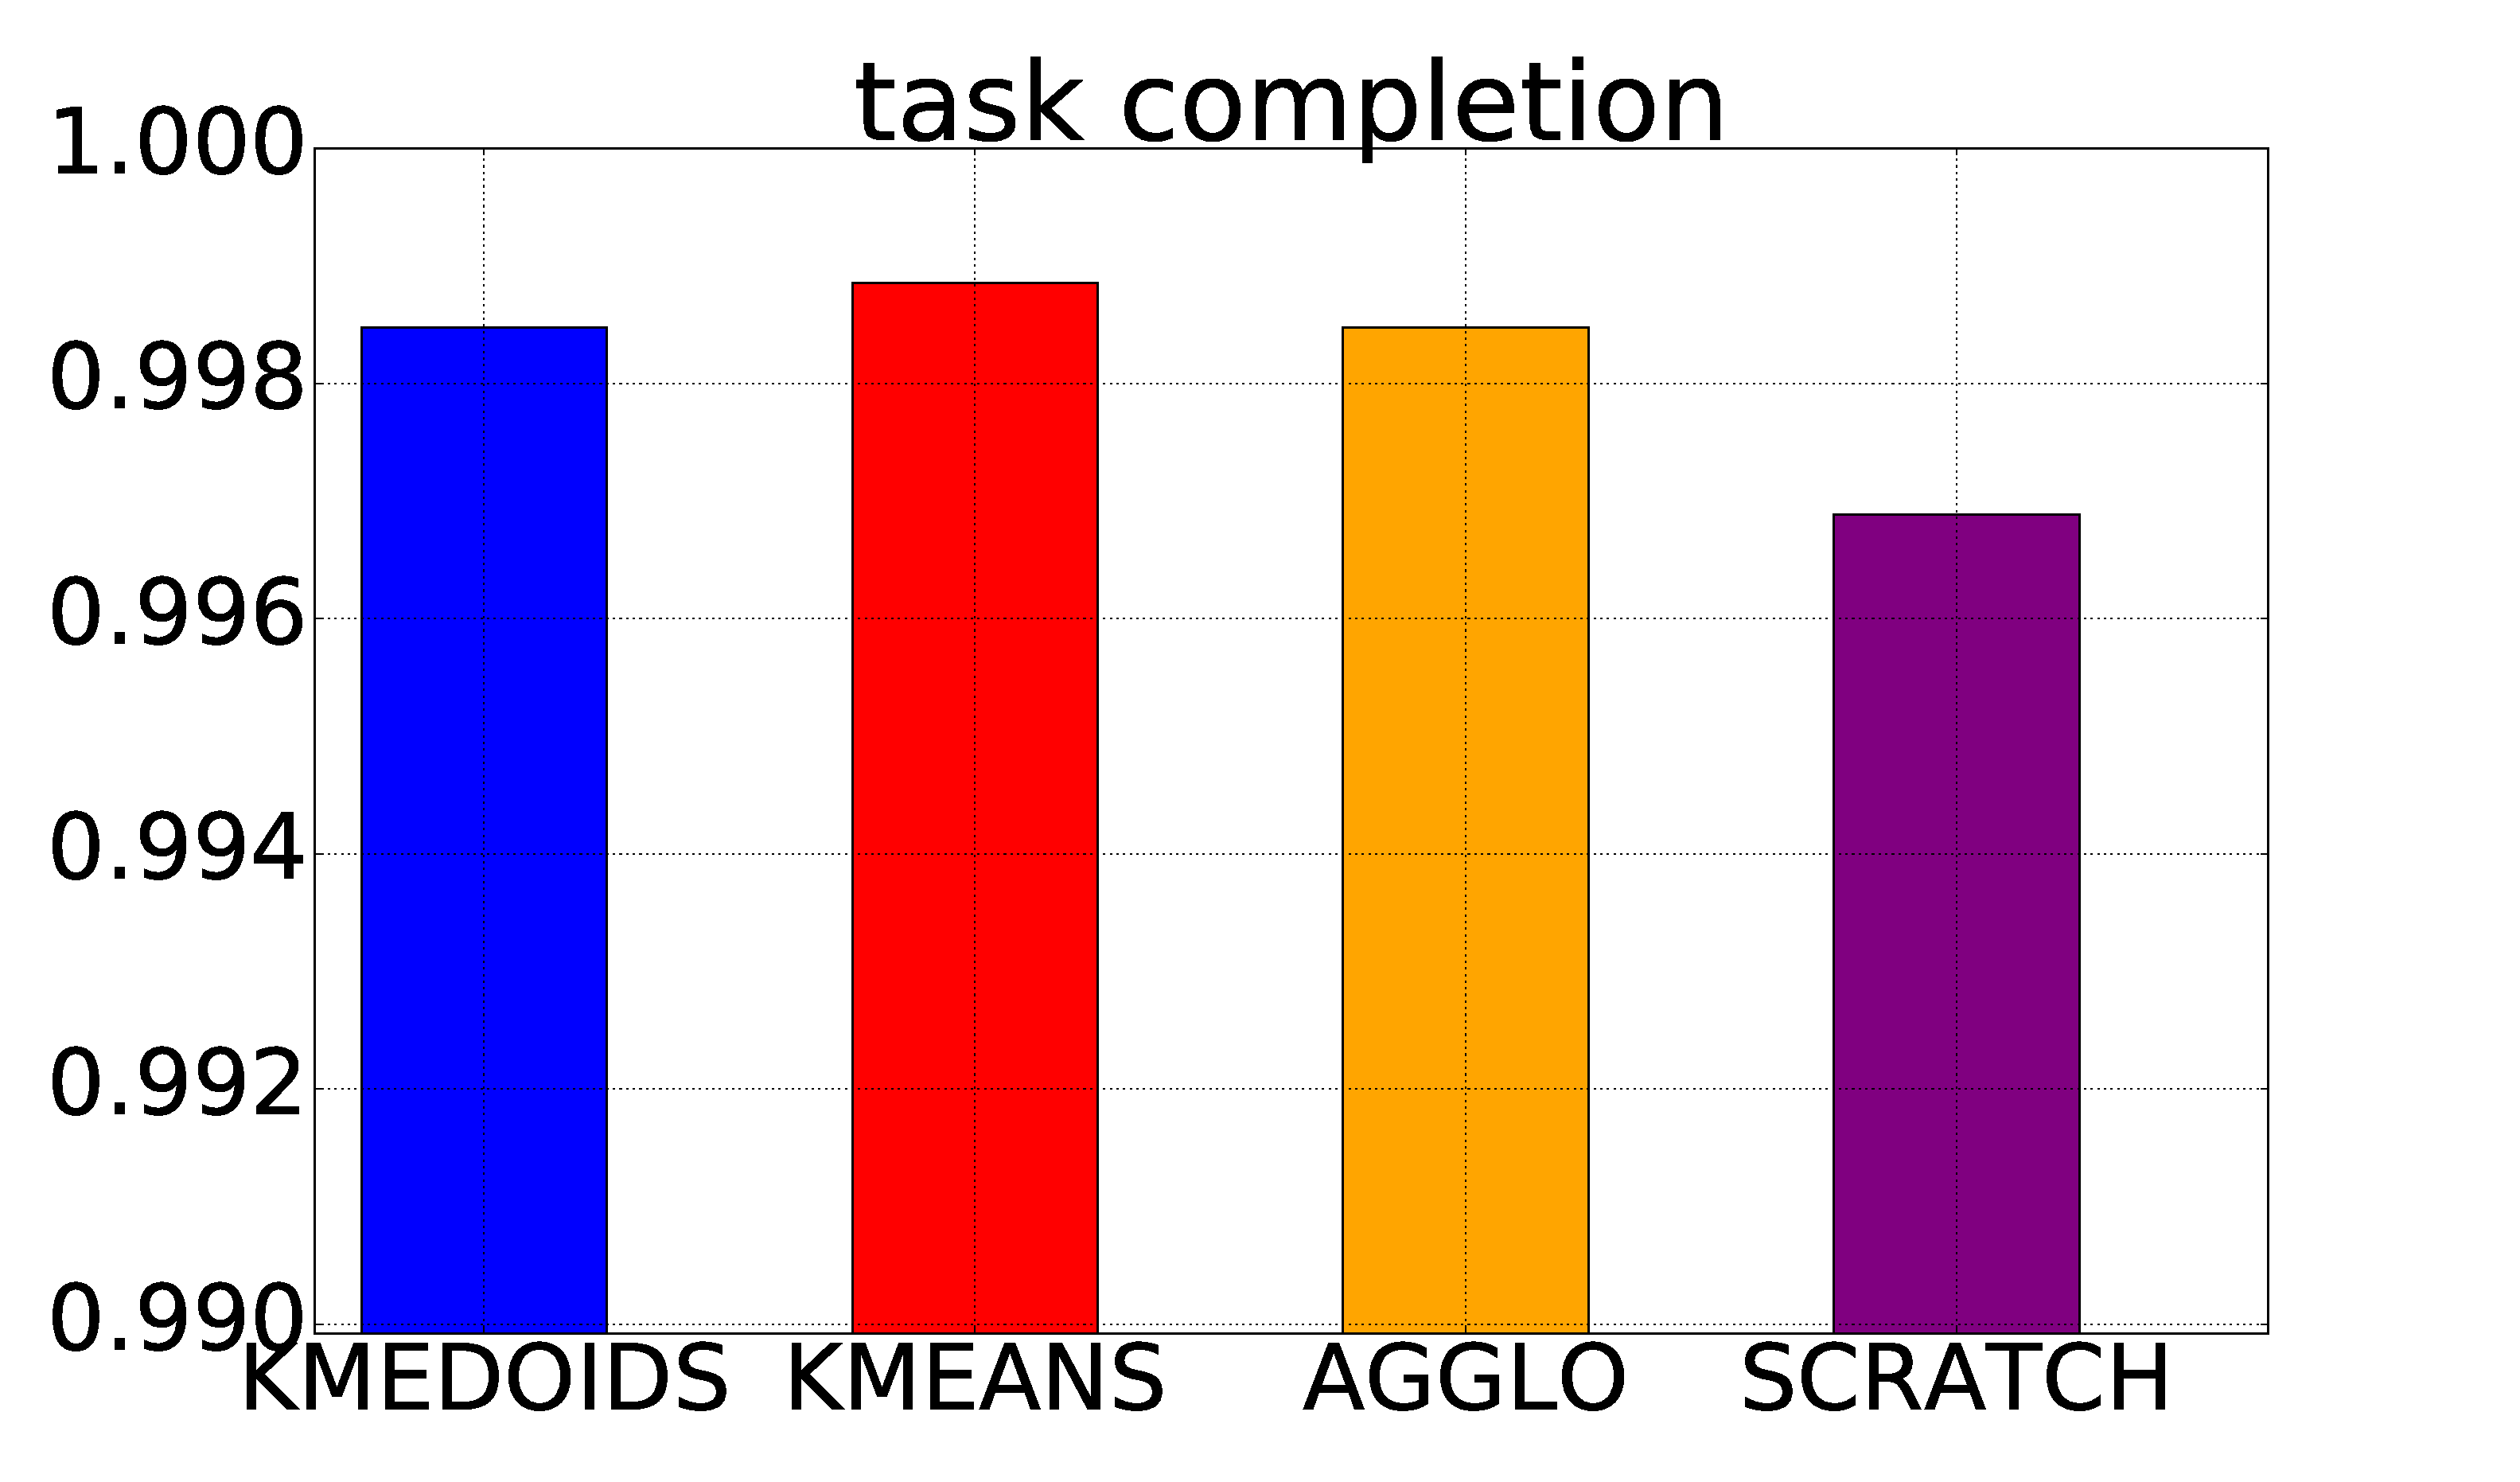
\includegraphics[width=0.5\textwidth]{img/humanTC.pdf}
                }
            \end{center}
        \end{figure}
    \end{frame}

    \begin{frame}{\textbf{Cross comparison} | human-model users}
        \begin{figure}
            \begin{center}
                \begin{tabular}{|l|c|c|c|c|c|}
                    \hline
                    \backslashbox{u}{s} & vsAlex & vsNico & vsWill & vsMerwan  \\
                    \hline
                    Alex & \textbf{1,074}   & 1,021 & 1,073 & 1,071        \\
                    Nico & 1,249 &     \textbf{1,251}     & 1,249 & 1,240    \\
                    Will & 1,126 & 1,104 &   \textbf{1,127}      & 1,120    \\
                    Merwan & 0,989 & 0,858 & 0,980 &    \textbf{ 0,998} \\
                    \hline
                \end{tabular}
            \end{center}
        \end{figure}
    \end{frame}


    \begin{frame}{\textbf{Cross comparison} | simulated users}
        \begin{figure}
            \begin{center}
                \setlength{\tabcolsep}{0.15em}
                \begin{tabular}{|l|c|c|c|c||c|c|c|c|c|c|c|c|c|}
                    \hline
                    \backslashbox{u}{s}& type & $c_{\top}$ & $c_{\bot}$ & x&vspu1 & vspu2 & vspu3 & vspu4 & vspu5 & vspu6 & vspu7   \\
                    \hline

                    pu1 & DU & 1 & -1 & 0.1 &  \textbf{0,62 }& 0,44 & 0,46 & 0,40 & 0,40 &0,40 & 0,59    \\
                    pu2 & DU & 5 & -5 & 0.1 & 0,53 &  \textbf{0,82}  & 0,81& 0,51 & 0,70 & 0,41 & 0,71 \\
                    pu3 & DU & 5 & -5 & 0.2& 0,53 &  \textbf{0,81} & \textbf{0,81}  & 0,52 & 0,72 & 0,42 & 0,71  \\
                    pu4 & RU & 5 & -5 & 0.1& 0,42 & 0,94 & 0,94 & \textbf{1,00}& 0,92 & 0,85 & 0,94 \\
                    pu5 & ARPBU & 1 & -1& &0,84& 0,98 & 1,00 & 1,11 &\textbf{1,16}& 1,13 & 1,05    \\
                    pu6 & AAU & 1 & -1 & &0,95 & 1,06 & 1,07 & 1,29 & 1,27 &\textbf{1,30} & 1,06 \\
                    pu7 & SAOTU & 1 & -1& &0,43 & 0,26& 0,27 & 0,10 & 0,18 & 0,03 &\textbf{ 0,58}  \\
                    \hline
                \end{tabular}
            \end{center}
        \end{figure}
    \end{frame}

    \begin{frame}
        \begin{itemize}
            \item (+) la solution fonctionne (en HDC)
            \item (.) heavily engineered
            \begin{itemize}
                \item (+) chaque composant peut être testé et validé
                \item (-) chaque composant générère des approximations et erreurs.
                \item (-) formulation complexe
                \item (-) meta paramètres
            \end{itemize}
        \end{itemize}

        Et si on pouvait:
        \begin{itemize}
            \item (+) une solution scalable naturellement
            \item (+) embarqué directement dans un algorithm "low level"
            \item (+) avec une formulation simple.
            \item $\rightarrow$ Solution: Transfer Deep Q-Learning (TDQN)
        \end{itemize}

    \end{frame}


    \subsection{Transfert continu}

    \foreach \n in {0}{%,1,2,3,4,5,6,7,8,9,10,11,12}{
    \begin{frame}{TDQN}

        \todo{overlay "won't work"}
        \begin{figure}
            \begin{center}
                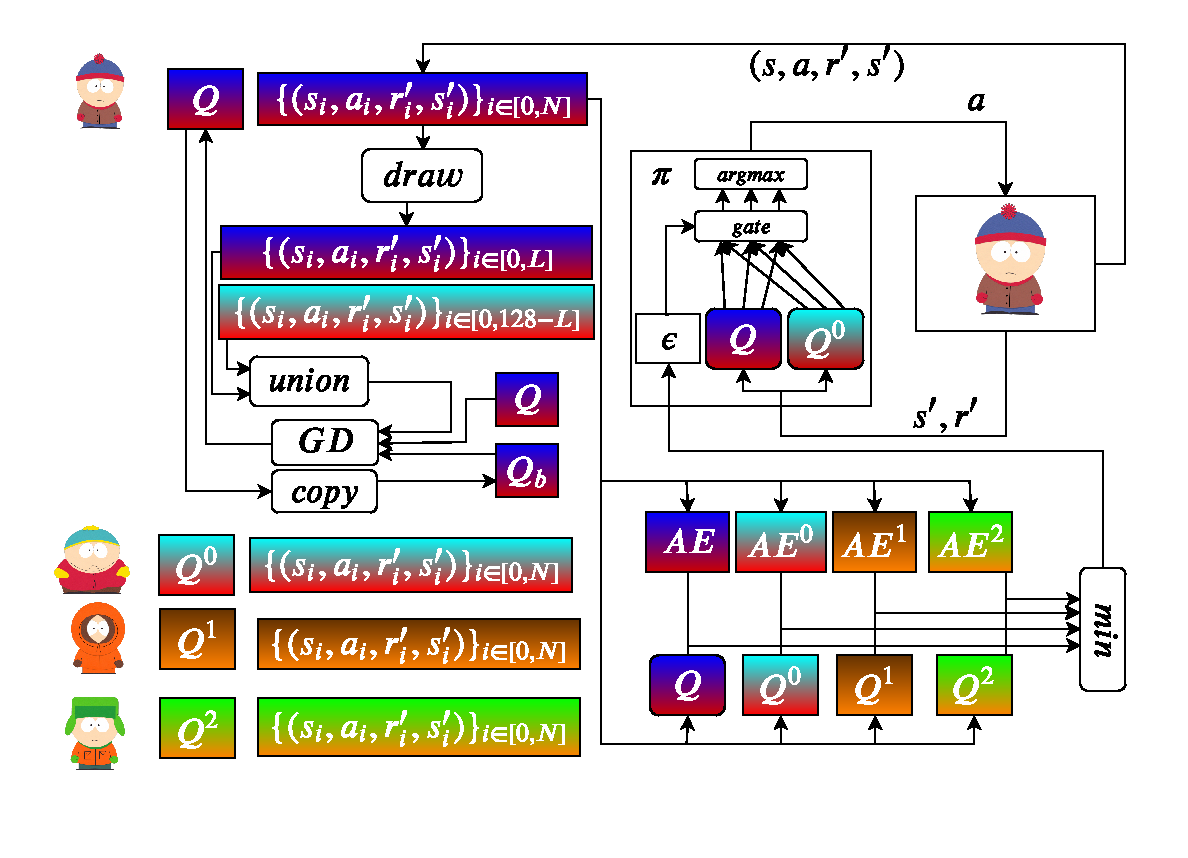
\includegraphics[width=1\textwidth]{img/tdqn1.pdf}
            \end{center}
        \end{figure}
    \end{frame}
    }

    \subsection{}

    \begin{frame}
        Le plus important dans un nouveau systèmes, c'est de garder l'user. Alors, au lieu d'optimiser, pourquoi ne pas focus sur le fait de pas le faire fuir ?
    \end{frame}

    \section{Apprentissage par transfert sécurisé}

    \subsection{epsilon safe}

    \begin{frame}
        On rajoute une info supplementaire (safery) lié intimement à la reception du signal de reward
        (+) peut donc guider l'apprentissage
        (+) d'une manière plus meta, eviter les dialogues trop catastrophiques pour eviter les dropouts.

    \end{frame}

    \begin{frame}

        \begin{figure}
            \begin{center}
                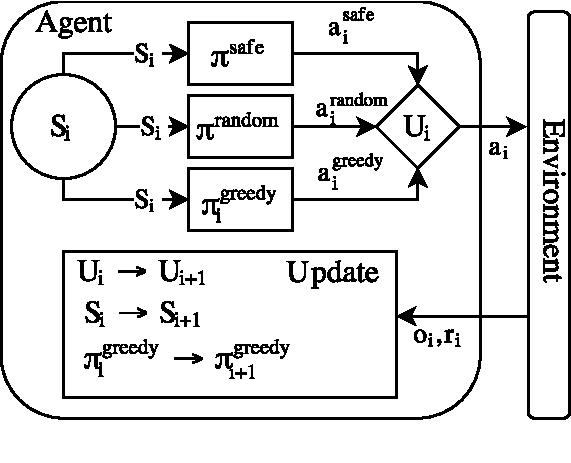
\includegraphics[width=0.5\textwidth]{img/transfer7.pdf}
            \end{center}
        \end{figure}

    \end{frame}

    \begin{frame}{Expériences}

        \todo{Expliquer l'environment et la FTQ lambda utilisé}
        \todo{Dire que l'autre FTQ (baseline) n'utilise pas le signal de contrainte}

    \end{frame}

    \begin{frame}{Expériences}

        \begin{figure}
            \captionsetup[subfigure]{labelformat=empty}
            \begin{center}
                \subfloat[Score du dialogue]{
                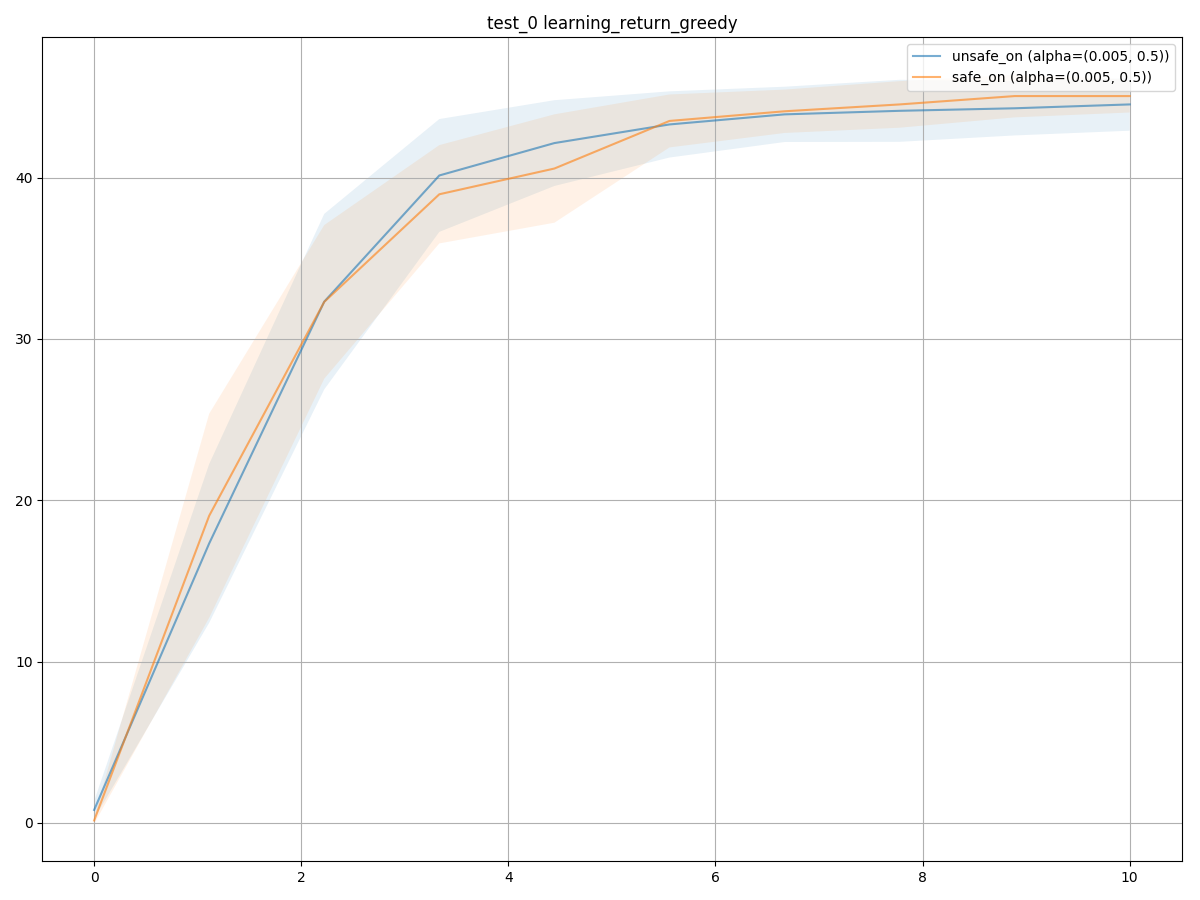
\includegraphics[width=0.5\textwidth]{img/retgreed.png}
                }
                \subfloat[Dialogue arrive à terme]{
                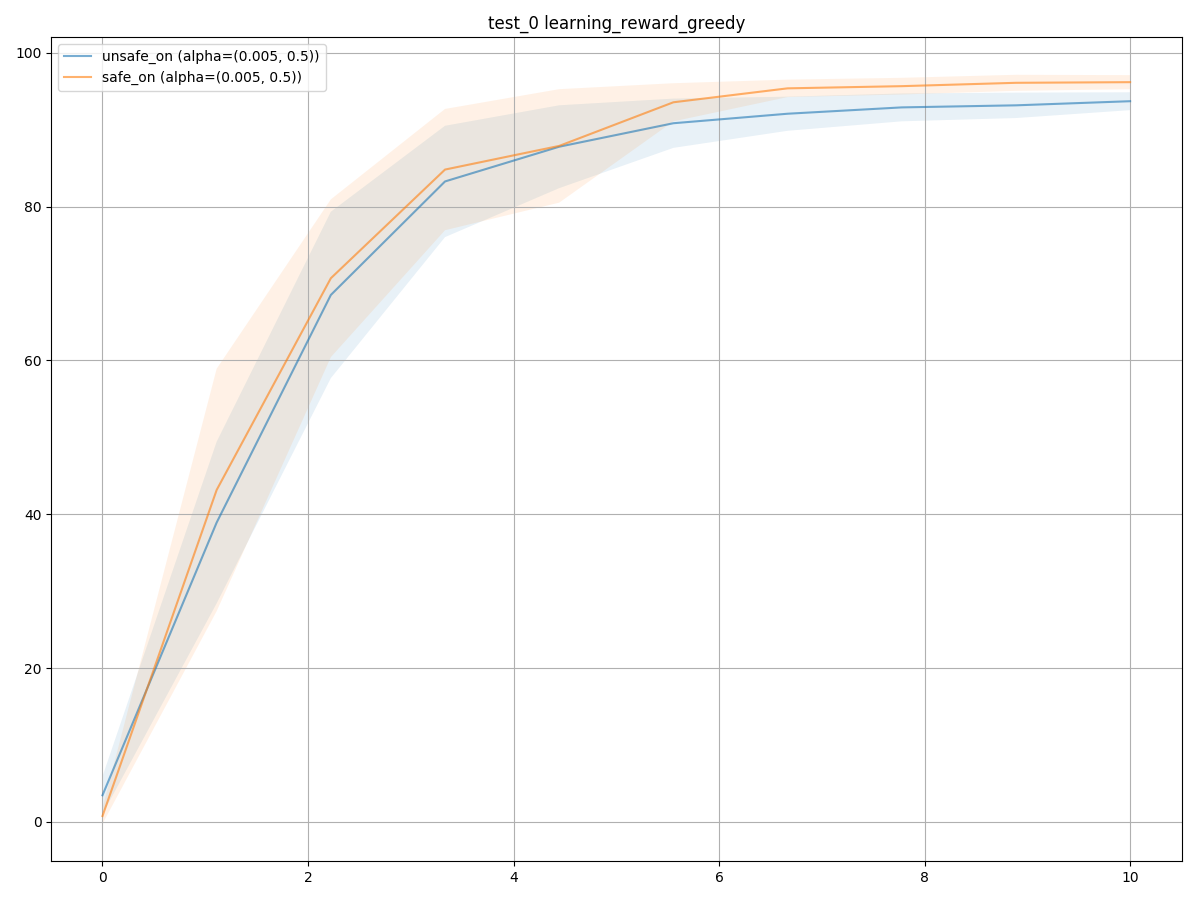
\includegraphics[width=0.5\textwidth]{img/rewgreed.png}
                }
            \end{center}
        \end{figure}


    \end{frame}
    \begin{frame}{Expériences}

        \begin{block}{Resultats}
            \begin{itemize}
                \item (+) Dialogues légérement plus sûr. % on garde donc l'user
                \item (-) mais cela n'affecte pas le score
                % et donc La vitesse d'apprentissage.
            \end{itemize}
        \end{block}

    \end{frame}
    \begin{frame}

        On a utilisé une politique lagragienne pour généré des dialogue safe.

        \begin{alertblock}{Limitation}
            La formulation linéaire de la reward implique des comportements extreme de $\pi_{safe}$: trop safe/trop risky.
            % et donc ça revient a avoir deux politiques greedy (ou lieu d'une safe+greedy)
        \end{alertblock}

        \begin{block}{Solution: calibration de lambda}% oral: limitation des politiques lagragiennes
            On cherche notre strategie safe sur le front de pareto
            \begin{itemize}
                \item (-) processus lourd et approximatif % où commencer, quel steps ?
                \item (-) il se peut qu'il n'existe meme pas de lambda
                % pas de formulation linéaire de la reward pour un budget donné
            \end{itemize}
        \end{block}

        \todo{Montrer un front de pareto: comment trouver la strategie associé à tel point sur le front ?}

        % Ce qui nous amène à la prochaine contribution.

    \end{frame}

    \subsection{Créer un système précautionneux, mais pas trop.}

    \begin{frame}{Des objectifs épurés}

        Ce qui nous interesse en réalité, c'est d'amasser des données personalisées sans perdre l'utilisateur.

        On propose d'utiliser une politique safe généralisée dès les premiers dialogues.

        Peut t on se contenter d'une politique lagragienne ? Non

    \end{frame}

    \begin{frame}

        \begin{block}{Solution: Constrainted Markov Decision Processes (CMDP)}
            \begin{itemize}
                \item (+) signal de contrainte en plus. DOF supplémentaire. On peut définir un budget de safety et d'afranchir des lambda.
                \item (-) si le budget change on the fly, ou qu'il n'est pas adapté, on doit reapprendre une politique
                \item (+) tractable
                \begin{itemize}
                    \item  Or Le front de pareto est rarement linéaire, le choix du budget n'est pas évident
                \end{itemize}
            \end{itemize}
        \end{block}
    \end{frame}

    \begin{frame}
        \begin{block}{Encore mieux: Budgeted Markov Decision Processes (BMDP)}
            \begin{itemize}
                \item (+) Formulation sous contraintes
                \item (+) Le budget est un paramètre du modèle (calcul le front de pareto)
                \item (-) \textit{Intractable}
            \end{itemize}
        \end{block}


    \end{frame}




    \begin{frame}
        \printbibliography[heading=bibempty]

    \end{frame}

\end{document}

